\documentclass[12pt,a4paper,twoside,openright,english]{book}
%**************************************************************
% Packages
%**************************************************************
\usepackage[utf8]{inputenc}
\usepackage[T1]{fontenc}
%\usepackage[latin1]{inputenc}
\usepackage[italian]{babel}
\usepackage{graphicx}
\usepackage{float}
\usepackage[toc, acronym]{glossaries}
\usepackage[nottoc]{tocbibind}
\usepackage{transparent}
\usepackage{hyperref}
\usepackage{color}
\usepackage{epstopdf}
\usepackage{subcaption}
\usepackage{wrapfig}
\usepackage{tikz}
%\usepackage{tikz-uml}
%\usepackage{fancyhdr}
\usepackage{rotating}
\usepackage{listings,lstautogobble}
\usepackage{glossaries}
\usepackage{enumitem}



\definecolor{bluekeywords}{rgb}{0,0,1}
\definecolor{greencomments}{rgb}{0,0.5,0}
\definecolor{redstrings}{rgb}{0.64,0.08,0.08}
\definecolor{xmlcomments}{rgb}{0.5,0.5,0.5}
\definecolor{types}{rgb}{0.17,0.57,0.68}



\colorlet{punct}{red!60!black}
\definecolor{background}{HTML}{EEEEEE}
\definecolor{delim}{RGB}{20,105,176}
\colorlet{numb}{magenta!60!black}


\lstdefinelanguage{json}{
	basicstyle=\normalfont\ttfamily,
	numbers=left,
	numberstyle=\scriptsize,
	stepnumber=1,
	numbersep=8pt,
	showstringspaces=false,
	breaklines=true,
	frame=lines,
	backgroundcolor=\color{background},
	literate=
	*{0}{{{\color{numb}0}}}{1}
	{1}{{{\color{numb}1}}}{1}
	{2}{{{\color{numb}2}}}{1}
	{3}{{{\color{numb}3}}}{1}
	{4}{{{\color{numb}4}}}{1}
	{5}{{{\color{numb}5}}}{1}
	{6}{{{\color{numb}6}}}{1}
	{7}{{{\color{numb}7}}}{1}
	{8}{{{\color{numb}8}}}{1}
	{9}{{{\color{numb}9}}}{1}
	{:}{{{\color{punct}{:}}}}{1}
	{,}{{{\color{punct}{,}}}}{1}
	{\{}{{{\color{delim}{\{}}}}{1}
	{\}}{{{\color{delim}{\}}}}}{1}
	{[}{{{\color{delim}{[}}}}{1}
	{]}{{{\color{delim}{]}}}}{1},
}


\lstset{language=[Sharp]C,
	%captionpos=b,
	%numbers=left, %Nummerierung
	%numberstyle=\tiny, % kleine Zeilennummern
	%frame=lines, % Oberhalb und unterhalb des Listings ist eine Linie
	aboveskip=3mm,
	belowskip=3mm,
	showspaces=false,
	showtabs=false,
	breaklines=true,
	showstringspaces=false,
	breakatwhitespace=true,
	escapeinside={(*@}{@*)},
	commentstyle=\color{greencomments},
	morekeywords={partial, var, value, get, set, Public, HttpResponseMessage, async, HttpStatusCode, private, string, List<T>,OrganizationData,Organization},
	keywordstyle=\color{bluekeywords},
	stringstyle=\color{redstrings},
	basicstyle={\ttfamily},
	columns=flexible,	
	breaklines=true,
	tabsize=4,
	autogobble=true
}

\usepackage{setspace}
%\linespread{0.5}

%\pagestyle{fancy}


\usetikzlibrary{calc,trees,positioning,arrows,chains,shapes.geometric,decorations.pathreplacing,decorations.pathmorphing,shapes,matrix,shapes.symbols,fit}



%**************************************************************
% Setup
%**************************************************************

% Line spaceing
\renewcommand{\baselinestretch}{1.5}

% Links color
\hypersetup {
	colorlinks=true,
	linkcolor=black,
	urlcolor=blue,
	citecolor=black
}

% Macros
%\newcommand{\bff}{\acrshort{bff}}

% Diagrams
\tikzset{
	>=stealth',
	punktchain/.style={
		rectangle, 
		rounded corners, 
		fill=yellow!20,
		draw=black, very thick,
		text width=10em, 
		minimum height=3em, 
		text centered, 
		on chain},
	line/.style={draw, thick, <-},
	element/.style={
		tape,
		top color=white,
		bottom color=blue!50!black!60!,
		minimum width=8em,
		draw=blue!40!black!90, very thick,
		text width=10em, 
		minimum height=3.5em, 
		text centered, 
		on chain},
	every join/.style={->, thick,shorten >=1pt},
	decoration={brace},
	tuborg/.style={decorate},
	tubnode/.style={midway, right=2pt},
}

%**************************************************************
% Cover
%**************************************************************
\newcommand{\myName}{Andrea \textsc{Venier}}
\newcommand{\myTitle}{Integrazione tra applicazioni web mediante microservizi RESTful}
\newcommand{\mySubTitle}{Ampliamento delle funzionalità\\ di un’applicazione di Project Management}
\newcommand{\myDegree}{Corso di Laurea in Informatica}
\newcommand{\myUni}{Università di Padova}
\newcommand{\myDepartment}{Dipartimento di Matematica}
\newcommand{\myProf}{Gilberto \textsc{Filè}}
\newcommand{\myLocation}{Padova}
\newcommand{\myAA}{2015-2016}
\newcommand{\myTime}{Dicembre 2016}
\newcommand{\myCompany}{Athesys s.r.l}
\newcommand{\glo}[1]{#1{\ped{G}}}



\makeglossary
%\makenoidxglossaries
%**************************************************************
% Glossary definition
%**************************************************************
\newglossaryentry{package} {
	name=package,
	description={ in informatica è, un raggruppamento di classi, metodi programmi, librerie e procedure che sono logicamente collegate tra di loro
	},
	plural=packages
}
\newglossaryentry{task} {
	name=task,
	description={ è un compito secondo la definizione dello standard ISO/IEC 12207
	},
	plural=tasks
}
\newglossaryentry{Gantt} {
	name=Gantt,
	description={  è un diagramma di supporto alla gestione dei progetti
	}
}
\newglossaryentry{custom} {
	name=custom,
	description={ è un attributo con cui si indica un manufatto, un dispositivo, o un componente, progettato e realizzato su misura in base alle necessità dell'acquirente o della funzione specifica che è destinato ad assolvere
	}
}
\newglossaryentry{APIg} {
	name={API},
	description={ è l'acronimo per Application Programming Interface (in italiano interfaccia di programmazione di un'applicazione), in informatica, indica ogni insieme di procedure disponibili al programmatore, di solito raggruppate a formare un set di strumenti specifici per l'espletamento di un determinato compito all'interno di un certo programma. Spesso con tale termine si intendono le librerie software disponibili in un certo linguaggio di programmazione
	}
}

\newglossaryentry{provider} {
	name=provider,
	description={ è un'espressione inglese che indica imprese che forniscono servizi di vario tipo,  italiano si è soliti tradurre "service provider" letteralmente, chiamando l'impresa "fornitore di servizi"
	},
	plural=providers
}
\newglossaryentry{token} {
	name=token,
	description={ con questo termine si fa riferimento ai Json Web Token (o JWT) che sono stringhe di caratteri alfanumerici che tipicamente incapsulano le credenziali di sicurezza per una sessione di login, identificando l'utente della stessa. Questi token sono segnati da una chiave del server grazie la quale è possibile verificarne la veridicità
	}
}
\newglossaryentry{header} {
	name=header,
	description={ o intestazione, è una parte del pacchetto ,inviato nelle richieste http, che contiene le informazioni di controllo necessarie al funzionamento della rete cioè le informazioni di protocollo aggiunte di strato in strato
	},
	plural=headers
}
\newglossaryentry{endpoint} {
	name=endpoint,
	description={ è l'url attraverso il quale un'applicazione client può accedere ad un servizio web. Lo stesso servizio web di solito ha endpoint multipli
	},
	plural=endpoints
}
\newglossaryentry{JSONg} {
	name={JSON},
	description={  acronimo di Javascript Object Notation, è un formato adatto all'interscambio di dati fra applicazioni client-server
	}
}

\newglossaryentry{REST-based} {
	name=REST-based,
	description={ fa riferimento ad architetture o chiamate  basate sul protocollo REST (vedi sez. \ref{rest})
	}
}
\newglossaryentry{JOIN} {
	name=JOIN,
	description={  è una clausola del linguaggio SQL che serve a combinare (unire) le tuple di due o più relazioni di un database tramite l'operazione di congiunzione (od unione) dell'algebra relazionale
	}
}
\newglossaryentry{SQL} {
	name=SQL,
	description={ è un linguaggio standardizzato per database basati sul modello relazionale
	}
}
\newglossaryentry{query} {
	name=query,
	description={ indica l'interrogazione da parte di un utente di un database, strutturato tipicamente secondo il modello relazionale, per compiere determinate operazioni sui dati
	},
	plural=queries
}
\newglossaryentry{framework} {
	name=framework,
	description={  architettura o struttura di supporto su cui un programma può essere creato. In genere è composto da una serie di librerie e strumenti di sviluppo
	},
	plural=frameworks
}
\newglossaryentry{virtual machine} {
	name=virtual machine,
	description={ o macchina virtuale (VM), viene indicato un software che, attraverso un processo di virtualizzazione, crea un ambiente virtuale che emula tipicamente il comportamento di una macchina fisica grazie all'assegnazione di risorse hardware
	},
	plural=virtual machines
}
\newglossaryentry{Design Pattern} {
	name=Design Pattern,
	description={ nell'ambito dell'ingegneria del software, un design pattern, è un concetto che può essere definito "una soluzione progettuale generale ad un problema ricorrente". Si tratta di una descrizione o modello logico da applicare per la risoluzione di un problema che può presentarsi in diverse situazioni durante le fasi di progettazione e sviluppo del software, ancor prima della definizione dell'algoritmo risolutivo della parte computazionale
	},
	plural=Design Patterns
}
\newglossaryentry{stateless} {
	name=stateless,
	description={ è un protocollo di comunicazione che tratta ogni richiesta come una transazione indipendente, scollegata da qualsiasi precedente richiesta, rendendo la comunicazione composta da coppie indipendenti di richiesta e risposta. Un protocollo stateless inoltre non richiede che il server mantenga le informazioni della sessione per ogni partner di comunicazione per la durata di multiple richieste
	}
}
\newglossaryentry{caching} {
	name=caching,
	description={ è il processo di immagazzinamento dati in una cache, che è una memoria temporanea
	}
}
\newglossaryentry{UML} {
	name=UML,
	description={ è un linguaggio di modellazione e specifica basato sul paradigma object-oriented
	}
}
\newglossaryentry{route} {
	name=route,
	description={ ci si riferisce alla definizione di un URI e a come esso risponde ad una specifica richiesta HTTP di un client
	},
	plural=routes
}
\newglossaryentry{generic} {
	name=generic,
	description={ è un tipo di dato utilizzato negli algoritmi di programmazione che non ha la necessità di essere istanziato immediatamente, bensì può essere specificato in un secondo momento
	},
	plural=generics
}
\newglossaryentry{accessor} {
	name=accessor,
	description={per il linguaggio di programmazione C\# un accessor di una proprietà (o campo dati di una classe) contiene il codice associato con l'operazione di \textit{getting} (lettura) o il \textit{setting} (scrittura) della proprietà stessa. La dichiarazione un un accessor può contenerne uno di tipo \textit{get}, uno di tipo \textit{set} o entrambi
	},
	plural=accessors
}
\newglossaryentry{getter} {
	name=getter,
	description={ è un metodo di una classe utilizzato per leggere il valore di un campo dati della stessa
	},
	plural=getters
}
\newglossaryentry{setter} {
	name=setter,
	description={ è un metodo di una classe utilizzato per scrivere il valore di un campo dati della stessa
	},
	plural=setters
}

\newglossaryentry{URLg} {
	name={URL},
	description={ o Uniform Resource Locator è una sequenza di caratteri che identifica univocamente l'indirizzo di una risorsa in Internet, tipicamente presente su un host server
	}
}
\newglossaryentry{Debugger} {
	name=Debugger,
	description={ è un programma/software specificatamente progettato per l'analisi e l'eliminazione dei bug (debugging), ovvero errori di programmazione interni al codice di altri programmi. E' spesso compreso all'interno di un ambiente integrato di sviluppo (IDE)
	},
	plural=Debuggers
}
\newglossaryentry{logging} {
	name=logging,
	description={ è la registrazione sequenziale e cronologica delle operazioni effettuate, da un utente, un amministratore o automatizzate, man mano che vengono eseguite dal sistema o applicazione
	}
}

\newglossaryentry{asset} {
	name=asset,
	description={ è una risorsa di un azienda
	}
}


\newglossaryentry{URIg} {
	name={URI},
	description={ o Uniform Resource Identifier, in informatica, si riferisce a una stringa che identifica univocamente una risorsa generica che può essere un indirizzo Web, un documento, un'immagine, un file, un servizio, un indirizzo di posta elettronica, ecc
	}
}

\newglossaryentry{cloud-based} {
	name=cloud-based,
	description={ si indica un paradigma basato, sul Cloud, di erogazione di risorse informatiche, come l'archiviazione, l'elaborazione o la trasmissione di dati, caratterizzato dalla disponibilità on-demand attraverso Internet a partire da un insieme di risorse preesistenti e configurabili
	}
}

%**************************************************************
% Acronyms definitions
%**************************************************************
\newacronym{CRM}{CRM}{Customer relationship management}

%\newacronym{JSON}{JSON}{JavaScript Object Notation}

\newacronym{http}{HTTP}{Hypertext Transfer Protocol}

\newacronym{DAO}{DAO}{Data Access Object}

\newacronym{DTO}{DTO}{Data Transfer Object}

%\newacronym{URI}{URI}{Uniform Resource Identifier}





%%% define the acronym and use the see= option
\newglossaryentry{URI}{type=\acronymtype, name={URI}, description={Uniform Resource Identifier}, first={Uniform Resource Identifier (URI)\glsadd{URIg}}, see=[Glossary:]{URIg}}

\newglossaryentry{JSON}{type=\acronymtype, name={JSON}, description={JavaScript Object Notation}, first={JavaScript Object Notation (JSON)\glsadd{JSONg}}, see=[Glossary:]{JSONg}}

\newglossaryentry{API}{type=\acronymtype, name={API}, description={Application Programming Interface}, first={Application Programming Interface (API)\glsadd{APIg}}, see=[Glossary:]{APIg}}

\newglossaryentry{URL}{type=\acronymtype, name={URL}, description={Uniform Resource Locator}, first={Uniform Resource Locator (URL)\glsadd{URLg}}, see=[Glossary:]{URLg}}

\title{\myTitle}
\author{\myName}
\date{\today}

\begin{document}

%**************************************************************
% Cover
%**************************************************************
\frontmatter
\begin{titlepage}
	\begin{center}
		\vbox to40pt{\vbox to\textheight{\vfill {\transparent{0.2}
\includegraphics[width=10cm]{logo-unipd.png}} \vfill}}
	\end{center}
	\begin{minipage}{.20\textwidth}
		
\includegraphics[height=2cm]{logo-department.png}
	\end{minipage}
	\hspace{40pt}
	\begin{minipage}{.80\textwidth}
		\begin{center}
			\begin{LARGE}
				\textsc{\textbf{\myUni}}\\
			\end{LARGE}
			\line(1,0){220}\\
			\begin{Large}
				\textsc{\myDepartment}\\
			\end{Large}
		\end{center}
	\end{minipage}
	\begin{center}
		\vfill
		\large{\textsc{\myDegree}}\\			
		\LARGE{\textsc{\textbf{\myTitle}}}\\
		\large{\mySubTitle}\\
		\vfill
		\begin{minipage}{0.4\textwidth}
			\begin{flushleft} \large
				\emph{Autore}\\
				\myName
			\end{flushleft}
		\end{minipage}
		\hfill
		\begin{minipage}{0.4\textwidth}
			\begin{flushright} \large
				\emph{Relatore} \\
				\myProf
			\end{flushright}
		\end{minipage}
		\vfill
		\line(1, 0){338} \\
		\begin{normalsize}
			\textsc{Anno Accademico \myAA}
		\end{normalsize}
	\end{center}
\end{titlepage}

%**************************************************************
% Colophon
%**************************************************************
\thispagestyle{empty}
\hfill
\vfill
\noindent \myName\ \textit{\myTitle,} \myDegree, Copyright \textcopyright\ \myTime.

\cleardoublepage
%\begingroup\onehalfspacing


%**************************************************************
% Keywords
%**************************************************************
\chapter*{Keywords}\label{keywords}
\paragraph*{CRM}
sta per \textit{Customer relationship management} e rappresenta un approccio per gestire le interazioni di un azienda con i suoi clienti, attuali e potenziali.\\
Attraverso questa metodologia si punta a raccogliere e analizzare i dati relativi ai cliente (email, sito aziendale, numeri telefonici ed in particolar modo lo storico delle offerte e degli ordini effettuati) con il fine di incrementare le vendite grazie alla fidelizzazione dello stesso mediante offerte e sconti mirati.\\
Seguendo questi concetti sono nati, e si sono affermati, diversi software CRM e tra i maggiori esponenti possiamo trovare: \textbf{Salesforce} e \textbf{Microsoft Dynamics}.\\
L'azienda \large{\myCompany{}}, basandosi sull'importanza e sulla diffusione dei suddetti software ha deciso di integrarli nella propria applicazione web di \textit{Project Management}.
 
\paragraph*{Project Management Software}
La disciplina di \textit{Project Management} si occupa di sovraintendere la pianificazione, l'organizzazione e l'implementazione di un progetto. Dove con progetto si intende un insieme ordinato di compiti da svolgere, caratterizzati da: vincoli di tempo (date di inizio e fine), risorse utilizzabili e risultati attesi.\\
Questa disciplina è fondamentale per controllare i costi, l'utilizzo delle risorse aziendali e per poter assicurare che il prodotto finale di questi processi soddisfi a pieno le esigenze del cliente.\\
In questo contesto \large{\myCompany{}} ha deciso di sviluppare \textbf{ADProject}, una soluzione software pensata ad-hoc per i propri clienti con l'obbiettivo di facilitare e automatizzare il suddetto insieme di attività.

%**************************************************************
% Abstract
%**************************************************************
\chapter*{Abstract}\label{abstract}
Questa tesi è basata sull'esperienza di stage che ho svolto presso l'azienda \textbf{Athesys s.r.l.}.
L’azienda \textbf{Athesys s.r.l.} ha costruito un software gestionale di Project Management, chiamato ADProject, che va ad integrare e ampliare le funzionalità di Microsoft Project, fornendo ai clienti la possibilità di avere un programma customizzato in base alle loro esigenze. ADProject permette di avere una panoramica costantemente aggiornata dei progetti presenti e passati dell’azienda, consente di spostare e assegnare risorse su determinati task di progetto, rendicontare il lavoro svolto dal personale ed inoltre di tenere sotto controllo i costi e le scadenze. Il progetto di stage consta nel costruire un modulo software che vada ad ampliare le funzionalità fornite da ADProject attraverso l’integrazione con Salesforce. In questo modo con ADProject si riusciranno a fornire, non solo strumenti all’avanguardia per la gestione di progetto, ma si potranno avere dati costantemente aggiornati relativi ai clienti dell’azienda, facilitando la gestione con gli stessi e permettendo inoltre la loro fidelizzazione grazie a rapporti e trattamenti aziendali mirati.

%**************************************************************
% Table of contents, list of figures and list of tables
%**************************************************************
\tableofcontents
\listoffigures
\listoftables

\mainmatter

%**************************************************************
% Introduzione
%**************************************************************
\chapter{Il Progetto}\label{introduzione}
	\section{Scopo del progetto}
	Il progetto, per quanto stabilito nel piano di lavoro dello stage, comporta l'integrazione di \textit{ADProject} con \textit{Salesforce} ma, dato che la parte principale dell'applicazione è stata finita con 2 settimane di anticipo, si è deciso di integrare nel servizio \textit{\textbf{ADCrm}} anche un secondo CRM: \textit{\textbf{Microsoft Dynamics}}.
	Nei successivi capitoli verrà descritta l'integrazione con entrambi i sistemi e verranno spiegate le sfide riscontrate in questo progetto, tuttavia per evitare eccessive ripetizioni ci si concentrerà soprattutto sulle parti riguardanti \textit{\textbf{SalesForce}}.
	\section{Studio delle applicazioni CRM}
		\subsection{Autenticazione}
			Per avere l'accesso ai dati l'applicazione deve potersi autenticare presso i server di SalesForce e Dynamics ed entrambe le applicazioie permettono l'autenticazione attraverso protocollo OAuth2.0.
			\paragraph{OAuth2.0}
			E' un protocollo aperto che permettere, in maniera semplice e standard, di autenticare e autorizzare applicazioni web, mobile e desktop ad accedere ai dati che si vogliono esporre. Viene comunemente usato come un modo per autorizzare siti web o applicazioni ad accedere ad altri siti senza fornire direttamente le credenziali dell'utente.\\
			La scelta di questo protocollo è stata obbligata, dato che è l'unico metodo d'autenticazione esposto dai CRM, tuttavia è un ottima opzione in quanto permette di rendere più sicuro il sistema, limitando la quantità di dati sensibili salvati all'interno dell'applicazione; inoltre sgrava il sistema dalle procedure di cambio password dato che sono a carico del \glo{provider} OAuth (SalesForce e Dynamics).
			%TODO: da ricontrollare
			\paragraph{Authentication Flow}
			%In questo paragrafo viene descritta la 
		\subsection{Protocolli di interrogazione}
			Entrambi i CRM permettono l'interrogazione dei propri dati attraverso l'implementazione di protocolli \textit{REST-based}. Questi offrono anche la possibilità di mettere in relazioni dati differenti, in maniera simile al comportamento della clausola \glo{JOIN} per le \glo{query} \glo{SQL}, anche se con limitazioni.\\ 
			La sfida che si è presentata in quest'ambito è stata quella di trovare il modo migliore di recuperare tutti i dati necessari limitando al più possibile il numero di richieste http inviate ai CRM, in quanto ogni nuova richiesta effettuata aumenta il tempo di re-indirizzamento dei dati recuperati verso ADProject.
			SalesForce e Microsoft Dynamics sfruttano due protocolli molto diversi tra di loro:
			%TODO: migliorare
			\paragraph{SOQL}
			o \textit{\textbf{S}alesforce \textbf{O}bject \textbf{Q}uery \textbf{L}anguage} permette recuperare i della propria organizzazione da SalesForce. SOQL è basato su richieste http ad uno specifico \glo{endpoint}, al cui url viene accodata una \glo{query} simile a quelle formulate nel linguaggio \glo{SQL}. In caso di richiesta corretta, Il CRM risponde con i dati richiesti in formato \glo{JSON}.
			\paragraph{OData}
			E' un protocollo aperto (Open Data Protocol) creato da Microsoft, che definisce un insieme di best-practices per costruire e utilizzare API RESTful.\\
			Dynamics permette l'interrogazione dei propri dati attraverso semplici richieste http basate su questo protocollo, dando in risposta i dati richiesti in formato \glo{JSON}.
			
			
%**************************************************************
% Tecnologie e Strumenti
%**************************************************************
\chapter{Tecnologie e Strumenti}\label{tecnologie}
\section{Frameworks e linguaggi di programmazione}
In questa sezione verranno descritti brevemente i linguaggi di programmazione usati nella scrittura di \textbf{ADProject} e di \textbf{ADCrm}.
Non tutti i linguaggi che verranno presentati in seguito sono stati usati nell'ambito del progetto di stage (in quanto limitato alla realizzazione del servizio \large{ADCrm}), tuttavia la loro contestualizzazione all'interno dei vari moduli sviluppati dall'azienda aiuta a capire meglio il funzionamento degli stessi.

\paragraph{.NET Framework}
è un \glo{framework} software sviluppato da Microsoft. Include una vasta classe di librerie chiamata \textit{Framework Class Library} (FLC) che permette l'interoperabilità tra i linguaggi di programmazione del \glo{framework}. I programmi scritti per .NET vengono eseguiti in un ambiente software conosciuto come \textit{Common Language Runtime} (CLR), una \textit{virtual machine}  che fornisce servizi come la gestione delle eccezioni e la gestione della memoria. FCL e CLR insieme costituisco .NET.\\
Il software di project management \textbf{ADProject} e il modulo \textbf{ADCrm} sono sviluppati su questo \glo{framework}.
%TODO da incrementare questa parte o specificarla meglio

\paragraph{ASP.NET}
 è un \glo{framework} server-side, sviluppato da Microsoft, per la creazione di applicazioni web, che permette ai programmatori di costruire pagine dinamiche, applicazioni e web services.
 ASP.NET viene usato per lo sviluppo di tutte le pagine web dinamiche che fungono da interfacce grafiche per ADProject.

\paragraph{Visual Basic .NET}
è un linguaggio di programmazione orientato agli oggetti sviluppato su .NET.\\
Con questo linguaggio è stato sviluppato ADProject, e sono tuttora in sviluppo numerosi moduli di questo software. La motivazione principale che ha portato i developers assegnati al progetto a scegliere questo linguaggio è stata la loro familiarità con lo stesso. 

\paragraph{C\#}
è un linguaggio di programmazione orientato agli oggetti sviluppato su .NET.
La sintassi del linguaggio prende spunto da C++ , da Java
e da Visual Basic.
Questo linguaggio sta alla base di tutto lo sviluppo del microservice ADCrm,soggetto di questa tesi. La scelta si potrebbe pensare poco sensata in quanto ADCrm deve integrarsi con un applicazione web interamente scritta con Visual Basic .NET, tuttavia ci sono delle forti motivazioni che hanno fatto propendere il team di sviluppo ad adottare questo linguaggio:
\begin{itemize}
	\item avendo scelto di adottare una struttura basata su microservices per lo sviluppo di ADCrm, ed essendo quindi un modulo fisicamente slegato da ADProject, è possibile scegliere un linguaggio di programmazione differente da VB.NET, pur rimanendo all'interno dei linguaggi offerti dal \glo{framework};
	\item i programmatori assegnati allo sviluppo del progetto hanno maggiore familiarità con questo linguaggio;
	\item C\# ha una vastissima comunity e mediamente è più facile reperire documentazione e teamplate rispetto a VB.NET;
	\item è più probabile trovare futuri developer C\#, in caso di incremento e manutenzione di ADCrm.	
\end{itemize}

\section{Ambiente di sviluppo}
\paragraph{Visual Studio}
 è un potente l'ambiente di sviluppo multipiattaforma fornito da Microsoft ed è stata la scelta naturale per lo sviluppo di ogni componente di ADProject ed ADCrm.
Visual Studio supporta, oltre ai linguaggi e \glo{framework} sopracitati: C, C++, F\#, Html e Javascript. 
%TODO da specificare cosa vuol dire multipiattaforma

\chapter{Analisi}\label{analisi}

%**************************************************************
% Casi d'uso
%**************************************************************
\section{Casi d'uso}\label{usecase}
%TODO: da aggiungere alla tabella dei casi d'uso le precondizioni da ricontrollare le immagini se sbordano e da controllare se aggiungere testo all'inizio di questa sezione
I casi d'uso sono creati secondo lo standard UML 2.4 e sono identificati dalla seguente notazione:
\begin{center}
	UC[Codice]: [Titolo]
\end{center}
dove il \textbf{codice} è un numero progressivo identificativo di ogni requisito, gerarchico nel  caso di sotto-casi d'uso tramite la notazione \textit{CodiceUCPadre.CodiceSottoUC}. Per ogni caso d'uso deve inoltre essere indicato:
\begin{itemize}
	\item \textbf{Titolo:} breve ma non ambiguo
	\item \textbf{Attori:} principali e secondari coinvolti
	\item \textbf{Descrizione:} una descrizione sintetica del caso d'uso
	%\item \textbf{Precondizione:} condizione necessaria affinché il caso d'uso possa avvenire
	\item \textbf{Flusso principale degli eventi:} descrizione, eventualmente per punti, del main scenario del Caso d'uso
	\item \textbf{Postcondizione:} condizione del sistema dopo che il caso d'uso è avvenuto
\end{itemize}
\begin{small}

	\hypertarget{UC1}{}
	\subsection{Caso d'uso UC1: Configurazione Aziendale}
	
	\begin{figure}[H]
		\centering
		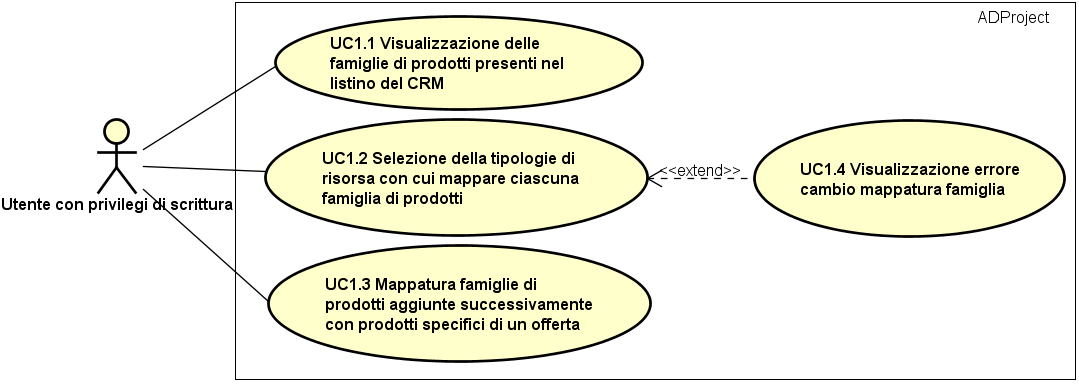
\includegraphics[scale=0.55]{images/useCase/UC1}
		\caption{Use Case 1 - Configurazione aziendale}
		%\caption{}
		\label{fig:uc1}
	\end{figure}
	\begin{longtable}{ | p{2.7cm} | p{12cm} |}
		\hline \textbf{Attori} & Utente con privilegi di scrittura\\ 
		\hline \textbf{Precondizione} & L’utente deve essere autenticato, deve possedere i privilegi di configurazione aziendale e deve essere stato configurato il collegamento ad un CRM\\
		\hline \textbf{Descrizione} & Attraverso l’interfaccia di configurazione aziendale, l’utente coi permessi corretti è in grado di visualizzare le impostazioni riguardanti la configurazione aziendale e modificarle\\ 
		\hline \textbf{Scenario Principale} & \begin{enumerate}
			\itemsep-0.5em 
			\item L’utente visualizza la lista delle famiglie di prodotti presenti nel listino del CRM  (UC1.1);
			\item L’utente seleziona la tipologia di risorse con cui andare a mappare ciascuna famiglia di prodotti  (UC1.2);
			\item L’utente mappa eventuali famiglie di prodotti non mappate o prodotti specifici di un’offerta che non sono stati mappati  (UC1.3).
			
		\end{enumerate}
		\\ 
		\hline \textbf{Postcondizione} & Sono state visualizzate ed eventualmente modificate le associazioni tra le famiglie di prodotti e le tipologie di risorse\\ 
		\hline 
	\end{longtable}
	
	\hypertarget{UC1.2}{}
	\subsection{Caso d'uso UC1.2: Selezione della tipologie di risorsa con cui mappare ciascuna famiglia di prodotti}
	
	\begin{figure}[H]
		\centering
		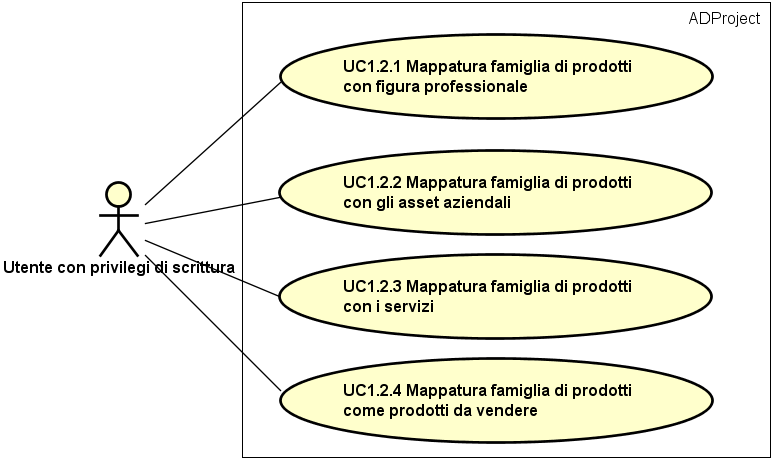
\includegraphics[width=\linewidth]{images/useCase/UC1_2}
		\caption{Use Case 1.2 - Mappatura tipologie risorse / famiglie prodotti}
		%\caption{}
		\label{fig:uc1.2}
	\end{figure}

	\begin{longtable}{ | p{2.7cm} | p{12cm} |}
		\hline \textbf{Attori} & Utente con privilegi di scrittura\\ 
		\hline \textbf{Precondizione} & L’utente deve essere autenticato, deve possedere i privilegi di configurazione aziendale e deve essere stato configurato il collegamento ad un CRM\\
		\hline \textbf{Descrizione} & Attraverso l’interfaccia di configurazione aziendale, l’utente coi permessi corretti è in grado di specificare con quale tipologia di risorsa (figura professionale, asset o servizio) dovrà essere mappata ciascuna tipologia di prodotto proveniente dal CRM\\ 
		\hline \textbf{Scenario Principale} & \begin{enumerate}
			\itemsep-0.5em 
			\item L’utente mappa una famiglia di prodotti con le figure professionali necessarie per un progetto  (UC1.2.1);
			\item L’utente mappa una famiglia di prodotti con gli asset necessarie per un progetto  (UC1.2.2);
			\item L’utente mappa una famiglia di servizi necessari per un progetto  (UC1.2.3);
			\item L’utente mappa una famiglia di prodotti come prodotti venduti (UC1.2.4).
			
		\end{enumerate}
		\\ 
		\hline \textbf{Estensioni} & \begin{enumerate}
			\item L’utente visualizza un messaggio di errore se tenta di cambiare la mappatura di una famiglia dopo che sono già stati importati prodotti relativi a quella famiglia  (UC1.4);
			
		\end{enumerate}
		\\ 
		\hline \textbf{Postcondizione} & Per almeno una famiglia di prodotto è stata modificata l’associazione ad una tipologia di risorsa. \\ 
		\hline 
	\end{longtable}
	
	\hypertarget{UC1.3}{}
	\subsection{Caso d'uso UC1.3: Mappatura famiglie di prodotti aggiunte successivamente con prodotti specifici di un offerta}
	\begin{figure}[H]
		\centering
		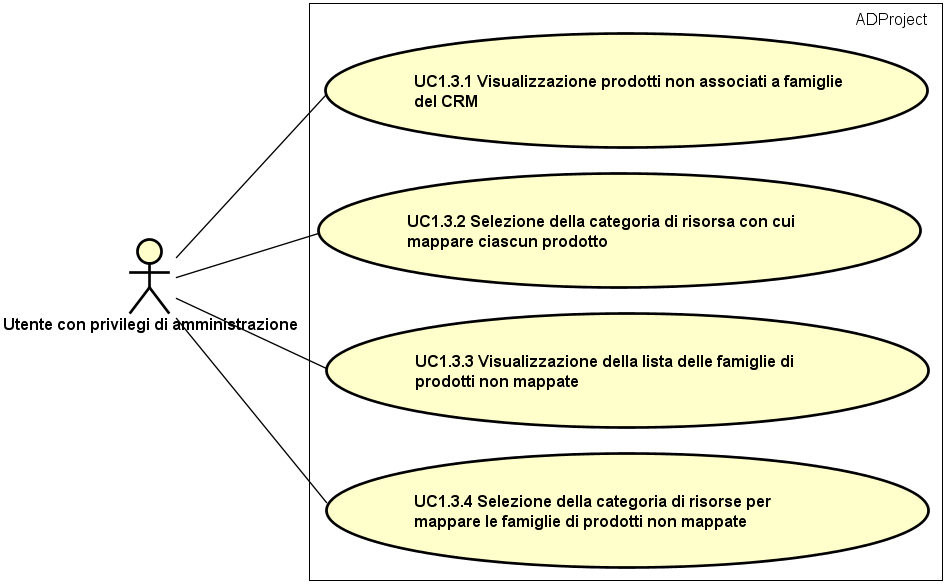
\includegraphics[scale=0.6]{images/useCase/UC1_3}
		\caption{Use Case 1.3 - Mappatura famiglie prodotti / prodotti offerta}
		%\caption{}
		\label{fig:uc1.3}
	\end{figure}
	\begin{longtable}{ | p{2.7cm} | p{12cm} |}
		\hline \textbf{Attori} & Utente con privilegi di scrittura\\
		\hline \textbf{Precondizione} &  L’utente deve essere autenticato, deve possedere i privilegi di configurazione di progetto, deve essere nella pagina di configurazione del progetto, deve aver selezionato il progetto e deve aver associato al progetto un’offerta che presenta prodotti con una mappatura anomala\\
		\hline \textbf{Descrizione} & Attraverso l’interfaccia di configurazione di progetto, l’utente coi permessi corretti è in grado di effettuare una mappatura \textit{just-in-time} di eventuali prodotti legati all’offerta che appartengono ad una famiglia di prodotti non mappata (perché ad esempio è stata aggiunta da poco nel CRM) o che non sono associati ad una famiglia (perché magari sono prodotti associati puntualmente all’offerta\\ 
		\hline \textbf{Scenario Principale} & \begin{enumerate}
			\itemsep-0.5em 
			\item L’utente visualizza la lista dei prodotti non associati ad alcuna famiglia del CRM  (UC1.3.1);
			\item L’utente seleziona la categoria di risorsa con cui mappare ciascun prodotto  (UC1.3.2);
			\item L’utente visualizza la lista delle famiglie di prodotti non mappate  (UC1.3.3);
			\item L’utente seleziona la categoria di risorsa con cui mappare ciascuna famiglia  (UC1.3.4).
			
		\end{enumerate}
		\\ 
		\hline \textbf{Postcondizione} & Sono state potenzialmente modificate le mappature dei prodotti\\ 
		\hline 
	\end{longtable}
	
	\hypertarget{UC2}{}
	\subsection{Caso d'uso UC2: Gestione delle anagrafiche aziendali}
	\begin{figure}[H]
		\centering
		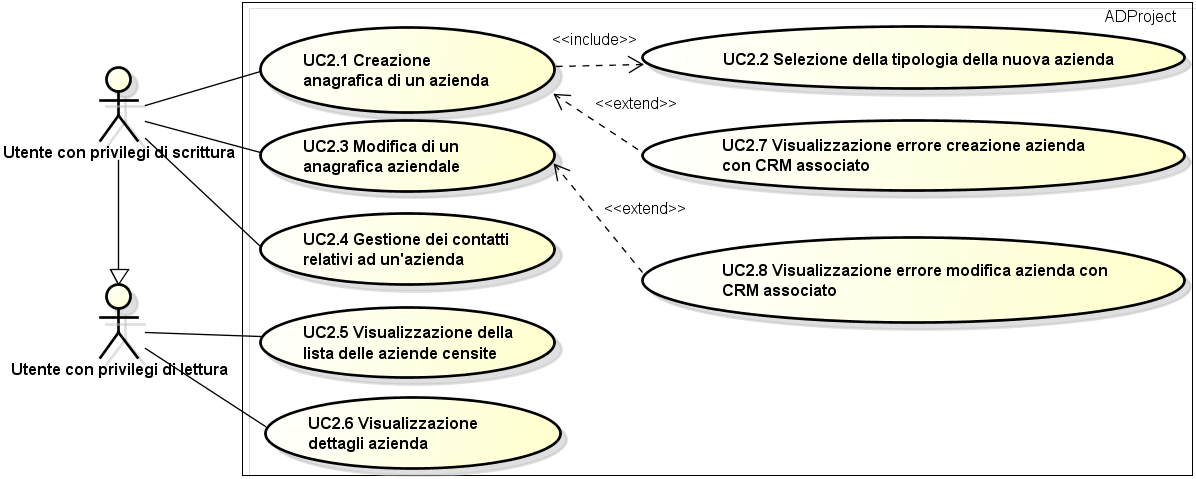
\includegraphics[scale=0.50]{images/useCase/UC2}
		\caption{Use Case 2 - Gestione anagrafiche aziendali}
		%\caption{}
		\label{fig:uc2}
	\end{figure}
	\begin{longtable}{ | p{2.7cm} | p{12cm} |}
		\hline \textbf{Attori} & Utente con privilegi di lettura, Utente con privilegi di scrittura\\
		\hline \textbf{Precondizione} &  L’utente deve essere autenticato, deve possedere almeno i privilegi di visualizzazione di configurazione di progetto. Non è necessario che l’applicazione sia collegata ad un CRM\\ 
		\hline \textbf{Descrizione} & Attraverso l’interfaccia di gestione delle anagrafiche aziendali, l’utente coi permessi corretti è in grado di visualizzare le informazioni relative alle schede di anagrafica aziendali e modificarle\\ 
		\hline \textbf{Scenario Principale} & \begin{enumerate}
			\itemsep-0.5em 
			\item L’utente crea un’anagrafica di un’azienda  (UC2.1);
			\item L’utente modifica l’anagrafica di un’azienda già censita  (UC2.3);
			\item L’utente gestisce i contatti relativi ad un’azienda  (UC2.4);
			\item L’utente visualizza la lista delle aziende censite nel sistema  (UC2.5);
			\item L’utente visualizza i dettagli relativi ad una azienda censita nel sistema  (UC2.6).
			
		\end{enumerate}
		\\ 
		\hline \textbf{Postcondizione} & Sono state visualizzate ed eventualmente modificate le anagrafiche aziendali\\ 
		\hline 
	\end{longtable}
	
	\hypertarget{UC2.4}{}
	\subsection{Caso d'uso UC2.4: Gestione dei contatti relativi ad un'azienda}
	\begin{figure}[H]
		\centering
		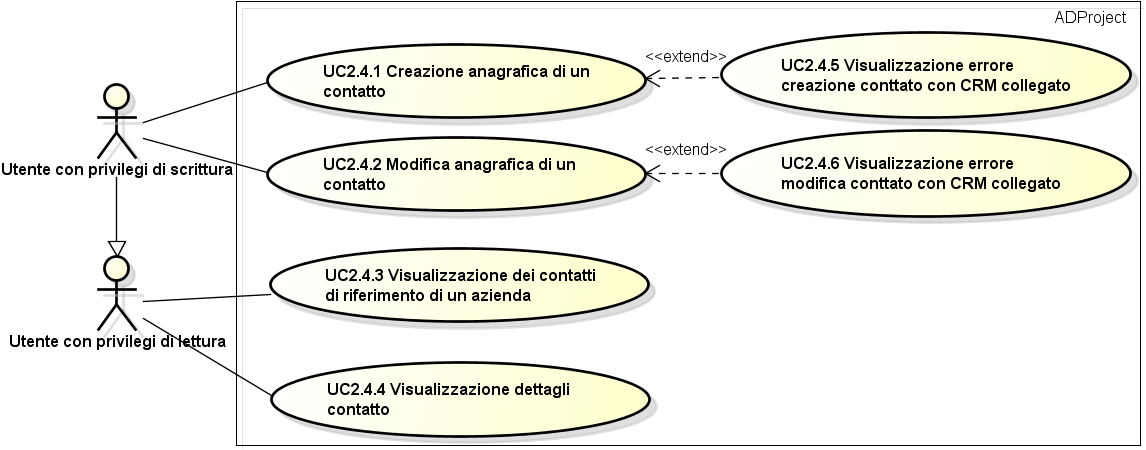
\includegraphics[scale=0.52]{images/useCase/UC2_4}
		\caption{Use Case 2.4 - Gestione contatti aziendali}
		%\caption{}
		\label{fig:uc2.4}
	\end{figure}
	\begin{longtable}{ | p{2.7cm} | p{12cm} |}
		\hline \textbf{Attori} & Utente con privilegi di scrittura\\
		\hline \textbf{Precondizione} &  L’utente deve essere autenticato, deve possedere almeno i privilegi di visualizzazione di configurazione di progetto. Non è necessario che l’applicazione sia collegata ad un CRM\\  
		\hline \textbf{Descrizione} & Attraverso l’interfaccia di gestione delle anagrafiche aziendali, l’utente coi permessi corretti è in grado di visualizzare le informazioni sui contatti di riferimento per le diverse aziende ed eventualmente modificarle\\ 
		\hline \textbf{Scenario Principale} & \begin{enumerate}
			\itemsep-0.5em 
			\item L’utente crea un’anagrafica di contatto ;
			\item L’utente modifica l’anagrafica di un contatto già censito ;
			\item L’utente visualizza la lista dei contatti di riferimento per una specifica azienda ;
			\item L’utente visualizza i dettagli relativi ad un contatto.
			
		\end{enumerate}
		\\ 
		\hline \textbf{Postcondizione} & Sono state visualizzate ed eventualmente modificate le informazioni relative ai contatti di riferimento per un’azienda\\ 
		\hline 
	\end{longtable}
	
	\hypertarget{UC3}{}
	\subsection{Caso d'uso UC3: Gestione dei progetti}
	\begin{figure}[H]
		\centering
		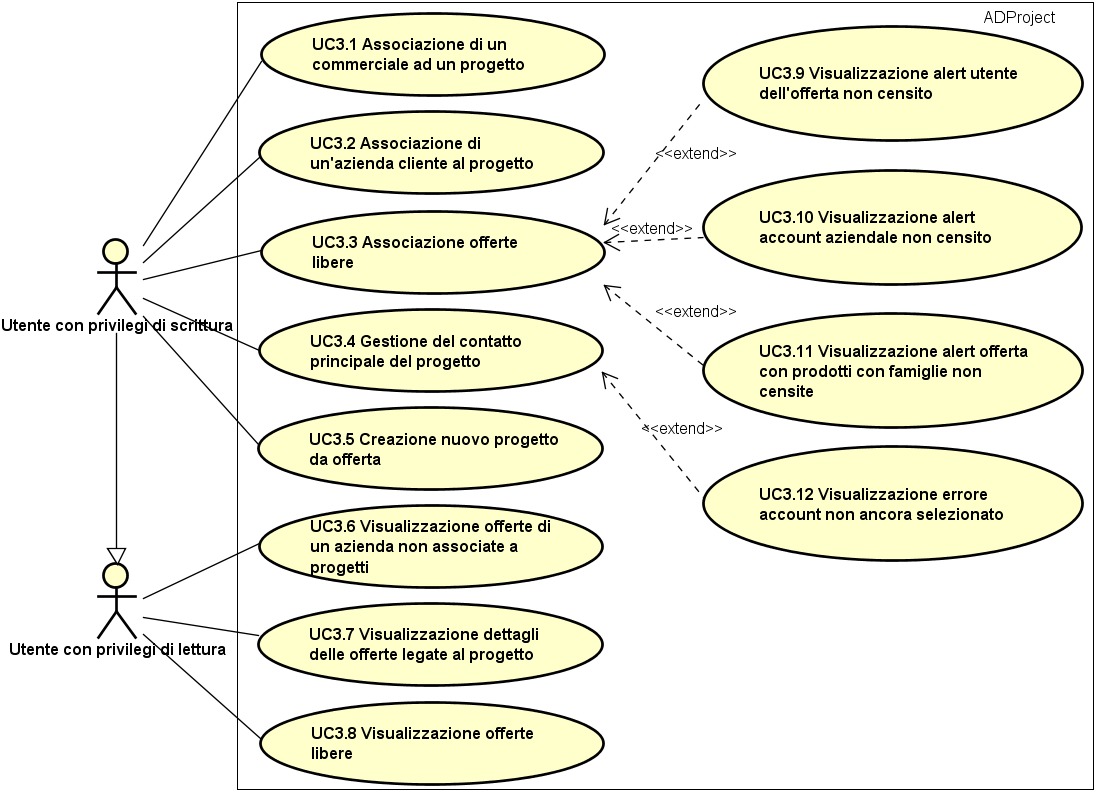
\includegraphics[scale=0.55]{images/useCase/UC3}
		\caption{Use Case 3 - Gestione progetti}
		%\caption{}
		\label{fig:uc3}
	\end{figure}
	\begin{longtable}{ | p{2.7cm} | p{12cm} |}
		\hline \textbf{Attori} & Utente con privilegi di lettura, Utente con privilegi di scrittura\\
		\hline \textbf{Precondizione} &  L’utente deve essere autenticato, possedere almeno i privilegi di visualizzazione di configurazione di progetto, essere nella pagina di configurazione del progetto, aver selezionato il progetto, il tipo del progetto non deve essere Interno. È necessario che l’applicazione sia collegata ad un CRM per quanto riguarda la parte relativa alle offerte\\  
		\hline \textbf{Descrizione} & Attraverso l’interfaccia di configurazione di progetto, l’utente coi permessi corretti è in grado di modificare le informazioni di progetto \\ 
		\hline \textbf{Scenario Principale} & \begin{enumerate}
			\itemsep-0.5em 
			\item L’utente associa un commerciale ad un progetto  (UC3.1);
			\item L’utente associa una delle aziende clienti censite al progetto  (UC3.2);
			\item L’utente associa una o più offerte libere al progetto selezionato  (UC3.3);
			\item L’utente gestisce il contatto principale di riferimento per un progetto  (UC3.4);
			\item L’utente visualizza la lista delle offerte libere (non associate ad alcun progetto) relative al cliente selezionato  (UC3.6);
			\item L’utente visualizza i dettagli delle offerte associate al progetto  (UC3.7);
			\item L’utente visualizza la lista di tutte le offerte libere  (UC3.8);
			\item L’utente può creare un progetto a partire da un’offerta  (UC3.5).
			
		\end{enumerate}
		\\ 
		\hline \textbf{Postcondizione} & Sono modificate le informazioni relative ad un progetto. \\ 
		\hline 
	\end{longtable}
	
	\hypertarget{UC3.4}{}
	\subsection{Caso d'uso UC3.4: Gestione del contatto principale del progetto}
		\begin{figure}[H]
		\centering
		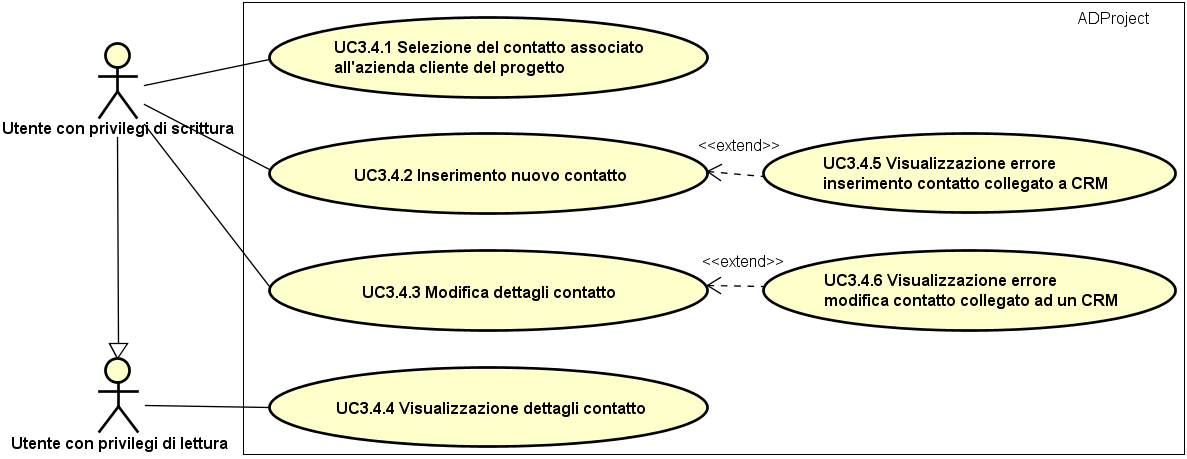
\includegraphics[scale=0.5]{images/useCase/UC3_4}
		\caption{Use Case 3.4 - Gestione contatto principale}
		%\caption{}
		\label{fig:uc3.4}
	\end{figure}
	\begin{longtable}{ | p{2.7cm} | p{12cm} |}
		\hline \textbf{Attori} & Utente con privilegi di scrittura\\
		\hline \textbf{Precondizione} &  L'utente ha selezionato la voce per gestire il contatto principale del progetto\\ 
		\hline \textbf{Descrizione} & Attraverso l’interfaccia di configurazione di progetto, l’utente coi permessi corretti è in grado di modificare le informazioni relative al contatto principale di riferimento per un progetto (il PM lato cliente)\\ 
		\hline \textbf{Scenario Principale} & \begin{enumerate}
			\itemsep-0.5em 
			\item L’utente seleziona uno dei contatti associato al cliente selezionato per il progetto  (UC3.4.1);
			\item L’utente inserisce un nuovo contatto  (UC3.4.2);
			\item L’utente modifica i dettagli relativi al contatto di riferimento per il progetto  (UC3.4.3);
			\item L’utente visualizza i dettagli relativi al contatto inserito  (UC3.4.4).
			
		\end{enumerate}
		\\ 
		\hline \textbf{Estensioni} & \begin{enumerate}
			\item Viene visualizzato un messaggio d'errore se si tenta di aggiungere un contatto principale prima che sia associato un'azienda cliente al progetto (UC3.12);
			
		\end{enumerate}
		\\ 
		\hline \textbf{Postcondizione} & Sono state modificate le informazioni relative al contatto principale di riferimento per un progetto \\ 
		\hline 
	\end{longtable}
	
	\hypertarget{UC3.5}{}
	\subsection{Caso d'uso UC3.5: Creazione nuovo progetto da offerta}
		\begin{figure}[H]
		\centering
		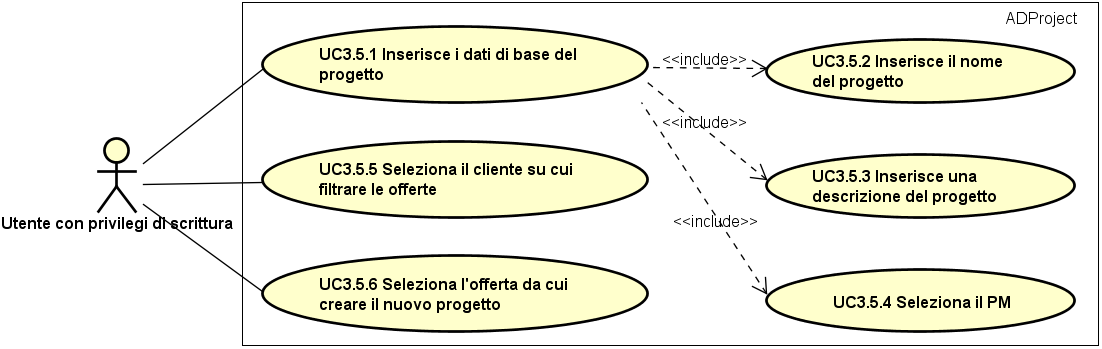
\includegraphics[scale=0.55]{images/useCase/UC3_5}
		\caption{Use Case 3.5 - Creazione progetto da offerta}
		%\caption{}
		\label{fig:uc3.5}
	\end{figure}
	\begin{longtable}{ | p{2.7cm} | p{12cm} |}
		\hline \textbf{Attori} & Utente con privilegi di scrittura\\ 
		\hline \textbf{Precondizione} &  L'utente selezionata la voce per creare un nuovo progetto partendo da un offerta esistente\\ 
		\hline \textbf{Descrizione} & L'utente crea un progetto a partire dai dati di una specifica offerta, auto-completando quindi l'associazione tra progetto con account, offerta e contatto\\ 
		\hline \textbf{Scenario Principale} & \begin{enumerate}
			\itemsep-0.5em 
			\item L’utente inserisce i dati di base del progetto  (UC3.5.1);
			\item L’utente selezione il cliente su cui filtrare le offerte  (UC3.5.2);
			\item L’utente seleziona l’offerta da cui creare il nuovo progetto  (UC3.5.3).
			
		\end{enumerate}
		\\ 
		\hline \textbf{Postcondizione} & Viene creato un nuovo progetto\\ 
		\hline 
	\end{longtable}
\end{small}





%**************************************************************
% Requisiti
%**************************************************************
\section{Requisiti}\label{requisiti}
Ogni requisito dovrà essere classificato per tipo e importanza, utilizzando la seguente struttura:
\begin{center}
	R[importanza][tipo][codice]
\end{center}
\begin{itemize}
	\item \textbf{Importanza} può assumere i seguenti valori:
	\begin{description}
		\item[1:] requisito desiderabile
		\item[2:] requisito opzionale
		\item[3:] requisito obbligatorio
	\end{description}
	\item \textbf{Tipo} può assumere i seguenti valori:
	\begin{description}
		\item[F:] Funzionale, descrive i servizi o le funzioni offerte dal sistema
		\item[Q:] Di Qualità, descrive i requisiti sulla qualità offerte dal sistema
		\item[P:] Prestazionale, descrive i requisiti sulle prestazioni offerte dal sistema
		\item[V:] Vincolo, descrive i vincoli sui servizi offerti dal sistema
	\end{description}
	\item \textbf{Codice} è un numero progressivo univoco per ogni requisito, indipendente da importanza e tipo. Nel caso si abbia un sotto-requisito codice può anche essere espresso in modo gerarchico tramite la notazione:
	\begin{center}
		\textit{CodiceRequistoPadre.CodiceSottorequisito}
	\end{center}
\end{itemize}
%Ogni requisito deve essere correlato da una sintetica ma precisa descrizione. Per ogni requisito bisogna indicarne le fonti, che posso essere il capitolato o uno o più casi d'uso.
%TODO: da controllare tutto e da controllare se aggiungere testo all'inizio di questa sezione
\begin{small}
\begin{longtable}{|r l|p{2.5cm}|p{10cm}|}
	\hline
	\multicolumn{2}{|c|}{\textbf{Codice}} & \textbf{Tipologia} & \textbf{Descrizione}\tabularnewline
	\hline
	& \hypertarget{R-3F1}{R-3F1} & Funzionale
	
	Obbligatorio & E' necessario avere un account con permessi amministrativi per Salesforce\tabularnewline
	\hline
	 & R-3F1.1 & Funzionale
	
	Obbligatorio & E' necessario che Salesforce sia configurato per esporre le API necessarie a recuperare i dati desiderati\tabularnewline
	\hline
	& \hypertarget{R-3F2}{R-3F2} & Funzionale
	
	Obbligatorio & L'applicazione ADCrm deve poter interrogare Salesforce attraverso le API RESTful che vengono esposte
	\tabularnewline
	\hline
	& R-3F2.1 & Funzionale
	
	Obbligatorio & L'applicazione ADCrm deve poter interrogare Salesforce per ottenere tutti i dati relativi alle Famiglie di Prodotti, recuperando: il campo identificativo della famiglia di prodotti, una descrizione della stessa ed un eventuale id del Parent\tabularnewline
	\hline
	 & R-3F2.2 & Funzionale
	
	Obbligatorio & L'applicazione ADCrm deve poter interrogare Salesforce per ottenere tutti i dati relativi agli Account delle aziende clienti recuperando: il campo identificativo, il nome e tutti i dati informativi riguardanti l'azienda (email,telefono,sito web,città,...)\tabularnewline
	\hline
	& R-3F2.3 & Funzionale
	
	Obbligatorio & L'applicazione ADCrm deve poter interrogare Salesforce per ottenere tutti i dati relativi ai contatti di un azienda recuperando: il campo identificativo, il nome, il cognome e tutti i dati informativi riguardanti il contatto (email, telefono, fax, ...)\tabularnewline
	\hline
	& R-3F2.4 & Funzionale
	
	Obbligatorio & L'applicazione ADCrm deve poter interrogare Salesforce per ottenere tutti i dati relativi alle offerte commerciali legate ad un azienda recuperando: il campo identificativo, l'identificativo aziendale, il prezzo, lo sconto e se l'offerta ha ordini associati \tabularnewline
	\hline
	& R-3F2.5 & Funzionale
	
	Obbligatorio & L'applicazione ADCrm deve poter interrogare Salesforce per ottenere tutti i dati relativi ai prodotti legati ad un offerta commerciale recuperando: il campo identificativo, il nome, la famiglia di prodotti a cui appartiene, l'identificativo dell'offerta, il prezzo, la quantità\tabularnewline
	\hline
	& R-3F2.6 & Funzionale
	
	Obbligatorio & L'applicazione ADCrm deve poter interrogare Salesforce per ottenere tutti i dati relativi agli utenti dell'azienda che utilizzano il CRM recuperando: il campo identificativo, il nome, il cognome e la email\tabularnewline
	\hline
	& R-3F3 & Funzionale
	
	Obbligatorio & L'applicazione ADCrm deve esporre delle API REST per poter essere interrogata da ADProject con il fine di fornire i dati recuperati\tabularnewline
	%%%%%%%%%%%%%%%%%%%%%%%%%%%%%%%%%%%%%%%%%%%%%%%%%%%%%%%%%
	\hline
	& \hypertarget{R-2F4}{R-2F4} & Funzionale
	
	Opzionale & E' necessario avere un account con permessi amministrativi per Microsoft Dynamics\tabularnewline
	\hline
	& R-2F4.1 & Funzionale
	
	Opzionale & E' necessario che Microsoft Dynamics sia configurato per esporre le API necessarie a recuperare i dati desiderati\tabularnewline
	\hline
	& \hypertarget{R-2F5}{R-2F5} & Funzionale
	
	Opzionale & L'applicazione ADCrm deve poter interrogare Microsoft Dynamics attraverso le API RESTful che vengono esposte
	\tabularnewline
	\hline
	& R-2F5.1 & Funzionale
	
	Opzionale & L'applicazione ADCrm deve poter interrogare Microsoft Dynamics per ottenere tutti i dati relativi alle Famiglie di Prodotti, recuperando: il campo identificativo della famiglia di prodotti, una descrizione della stessa ed un eventuale id del Parent\tabularnewline
	\hline
	& R-2F5.2 & Funzionale
	
	Opzionale & L'applicazione ADCrm deve poter interrogare Microsoft Dynamics per ottenere tutti i dati relativi agli Account delle aziende clienti recuperando: il campo identificativo, il nome e tutti i dati informativi riguardanti l'azienda (email,telefono,sito web,città,...)\tabularnewline
	\hline
	& R-2F5.3 & Funzionale
	
	Opzionale & L'applicazione ADCrm deve poter interrogare Microsoft Dynamics per ottenere tutti i dati relativi ai contatti di un azienda recuperando: il campo identificativo, il nome, il cognome e tutti i dati informativi riguardanti il contatto (email, telefono, fax, ...)\tabularnewline
	\hline
	& R-2F5.4 & Funzionale
	
	Opzionale & L'applicazione ADCrm deve poter interrogare Microsoft Dynamics per ottenere tutti i dati relativi alle offerte commerciali legate ad un azienda recuperando: il campo identificativo, l'identificativo aziendale, il prezzo, lo sconto e se l'offerta ha ordini associati \tabularnewline
	\hline
	& R-2F5.5 & Funzionale
	
	Opzionale & L'applicazione ADCrm deve poter interrogare Microsoft Dynamics per ottenere tutti i dati relativi ai prodotti legati ad un offerta commerciale recuperando: il campo identificativo, il nome, la famiglia di prodotti a cui appartiene, l'identificativo dell'offerta, il prezzo, la quantità\tabularnewline
	\hline
	& R-2F5.6 & Funzionale
	
	Opzionale & L'applicazione ADCrm deve poter interrogare Microsoft Dynamics per ottenere tutti i dati relativi agli utenti dell'azienda che utilizzano il CRM recuperando: il campo identificativo, il nome, il cognome e la email\tabularnewline
	\hline
	\caption{Tabella requisiti} 
	\tabularnewline
\end{longtable}

\end{small}
%**************************************************************
% Progettazione
%**************************************************************
\chapter{Progettazione}\label{progettazione}
In questo capitolo viene dettagliatamente descritta l'applicazione, presentando: 
\begin{enumerate}
	\itemsep-1em 
	\item I \glo{Design Pattern} utilizzati, contestualizzando il loro utilizzo;
	\item La descrizione dell'architettura ad alto livello del sistema;
	\item Le \glo{API} REST esposte per permettere al client di comunicare con l'applicazione;
	\item Una descrizione più dettagliata delle classi che rappresentano il cuore dell'applicazione.
\end{enumerate}

\section{Design pattern}\label{design_pattern}
\subsection{Microservices}
Lo stile architetturale a microservizi è un approccio per sviluppare una singola applicazione come un insieme di piccoli servizi autonomi che interagiscono tra di loro, ognuno dei quali gestisce i suoi processi e comunica attraverso meccanismi snelli, spesso \glo{API} http.
Questa architettura permette di velocizzare i tempi di sviluppo (essendo i servizi autonomi tra di loro essi possono raggiungere l'ambiente di produzione anche in momenti separati ed inoltre possono essere sviluppati da persone diverse), aumentare la resilienza del sistema (se uno dei servizi smette di funzionare essendo separato dagli altri, non pregiudica il funzionamento del sistema) ed è più facilmente scalabile rispetto ad un architettura monolitica.\\
Si è deciso di sviluppare ADCrm seguendo quest'ottica, ottenendo in questo modo:
\begin{itemize}
	\item una netta separazione dei compiti delle varie componenti del sistema;
	\item la possibilità di collegarsi a nuovi CRM senza dover modificare in alcun modo ADProject, in quanto esso comunica con il servizio attraverso un interfaccia comune;
	\item un aumento  della resilienza e la scalabilità dell'applicazione.
\end{itemize}


\subsection{RESTful}
REST o \textit{\textbf{Re}presentational \textbf{S}tate \textbf{T}ransfer} è un architettura software che permette di rendere interoperabili sistemi di computer attraverso internet. 
Un servizio web REST permette ai sistemi richiedenti, di accedere e manipolare una rappresentazione testuale delle sue risorse web attraverso un insieme predefinito di operazioni \glo{stateless}.
Utilizzare i metodi definiti per il protocollo http (GET, POST, PUT, DELETE) è il modo più comune accedere alle risorse web del sistema che le espone.
Questa architettura attraverso l'utilizzo del protocollo \glo{stateless} e di insiemi di operazioni standard, mira a garantire ottime performance, essere affidabile e scalabile senza dover necessitare di modificare tutto il sistema nel caso di cambiamenti a qualche sua componente.
L'architettura REST viene utilizzata da \textbf{ADCrm\textbf{}} per recuperare ed esporre a sua volta le risorse presenti sul CRM.
Concretamente sarà presente quindi un microservizio per ogni CRM che si vorrà collegare all'applicazione.

\subsection{DTO \& DAO}
Il DTO (\textit{Data Transfer Object}) e DAO (\textit{Data Access Object}) sono due design pattern architetturali spesso usati in congiunzione.\\
La loro funzione principale è quella di disaccoppiare il \textit{data layer} (la parte in cui risiedono i dati) dalla parte di \textit{business logic} (ciò che rappresenta la logica applicativa) dell'applicazione, aumentando cosi la separazione tra le varie componenti e quindi la loro modularità e manutenibilità.\\
Le classi di oggetti DTO al loro interno avranno solamente campi dati accedibili attraverso metodi \textit{getter} e \textit{setter}, mentre gli oggetti DAO implementeranno i metodi, utilizzati dalla \textit{business logic}, per accedere ai dati dell'applicazione utilizzando quindi i sopracitati \textit{Data Transfer Object}.

\subsection{Factory Method} \label{factory}
Questo design pattern creazionale, nell'ambito della programmazione orientata agli oggetti, permette di affrontare il problema della creazione di oggetti senza specificarne a priori l'esatta classe di appartenenza.
Il pattern fornisce un interfaccia per la creazione di un oggetto, ma lascia alle classi che la implementano la decisione di quale oggetto istanziare.\\

\begin{figure}[H]
	\centering
	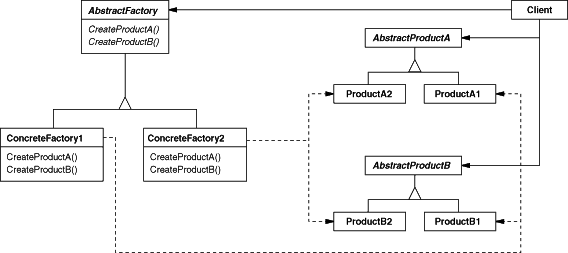
\includegraphics[width=\linewidth]{images/abstract_factory_structure}
	\caption{Schema UML d'esempio per il Factory design pattern}
	\label{fig:abstractfactorystructure}
\end{figure}

In questo modo l'applicazione ADCrm non solo non ha bisogno di sapere a priori se deve costruire oggetti per \textit{Salesforce} o altri CRM, ma ha anche la possibilità di aver collegarsi a più applicazioni CRM contemporaneamente.


\section{Architettura del sistema}
L'applicazione ADCrm presenta un'architettura client-server, assumendone entrambi i ruoli:
\paragraph{Server}
L'applicazione assume il ruolo di server nel momento in cui deve assolvere alle richieste che arrivano da ADProject mediante le API REST. Deve quindi rispondere a due esigenze principali:
\begin{itemize}
	\item esporre API REST per poter rispondere, in formato \glo{JSON}, alle richieste http ricevute;
	\item salvare i dati, non sensibili, necessari per il processo di autenticazione e collegamento con il CRM su un piccolo database interno.
\end{itemize} 

Si è deciso di mantenere il database sul servizio ADCrm per togliere l'onere ad ADProject di conoscere: non solo le procedure di autenticazione al CRM, ma anche la tipologia di CRM che si va ad interrogare (Salesforce, Dynamics, ...). In questo modo si riesce a mantenere una netta separazione dei ruoli tra le varie componenti. 

\paragraph{Client}
L'applicazione assume il ruolo di client nel momento in cui deve interrogare il server del CRM per recuperare i dati di cui ha bisogno ADProject, deve quindi:
\begin{itemize}
	\item interrogare il server remoto attraverso il set di API esposto;
	\item organizzare i dati ricevuti in modo tale che siano fruibili da ADProject;
	\item restituire gli stessi in formato \glo{JSON}.
\end{itemize}

Nelle prime fasi della progettazione si è valutata l'ipotesi di utilizzare un database per fare \glo{caching} dei dati provenienti dal CRM, così da limitare le richieste http necessarie e da velocizzare le risposte fornite, tuttavia la necessità di ADProject di utilizzare sempre dati aggiornati ha fatto abbandonare quest'opzione.\\

La figura \ref{fig:architetturasistema} illustra l'architettura ad alto livello del sistema; una descrizione più dettagliata delle varie componenti verrà esposta nelle sezioni successive.

\begin{figure}[H]
	\centering
	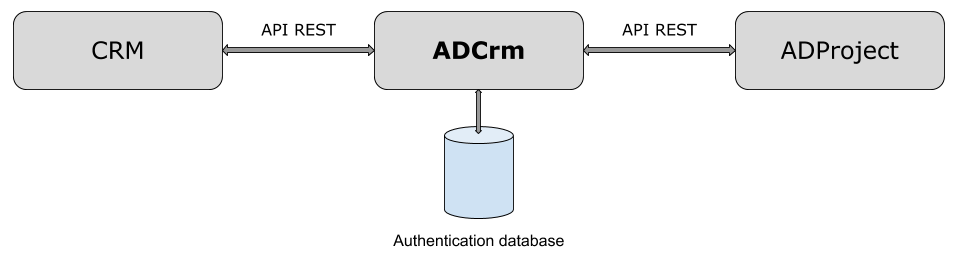
\includegraphics[width=\linewidth]{images/architettura_sistema}
	\caption{Architettura ad alto livello}
	\label{fig:architetturasistema}
\end{figure}

\section{API REST}\label{apiRest}
Di seguito si trova la definizione delle API REST esposte dal servizio ADCrm.\\
I metodi http con cui chiamare tutti i successivi URL sono metodi \textbf{GET} ed i dati ricevuti nelle risposte sono forniti in formato \glo{JSON}.

	\begin{small}
		\begin{longtable}{ | l | p{8cm} | }
			\hline \textbf{URL} & \textbf{Descrizione Risposta}\\
			\hline api/organization/\{organizationId\}/ & Risponde con i dati riguardante l'organizzazione avente \textit{id = organizationId}\\
			\hline
		\end{longtable}		
	\end{small}
Questo primo \glo{endpoint} necessita di ulteriori spiegazioni in quanto l'url specificato sopra è da anteporre a di tutti quelli che seguiranno (eg. "\textbf{api/organization/\{organizationId\}/accounts}" nel caso dell'url "/accounts").\\
Inoltre si noti che è necessario da parte di chi effettua chiamate verso questo url (e quindi anche verso tutti gli altri) conoscere il campo \textit{organizationId} per poter ottenere una risposta. Questa restrizione è stata posta per far si che il sistema sia più sicuro, rendendo disponibili dei dati riguardanti l'azienda fruitrice del servizio solo se si conosce il corretto identificativo.
%TODO: decidere se sistemare la parte qua sopra
	\begin{small}
		\begin{longtable}{ | l | p{8cm} | }
			\hline \textbf{URL} & \textbf{Descrizione Risposta}\\
			\hline /accounts & Risponde con la lista contenente i dati di tutti gli account\\
			\hline /accounts/\{\textit{accountId}\} & Risponde con i dati dell'account avente \textit{id = accountId}\\    
			\hline /accounts/\{\textit{accountId}\}/contacts & Risponde con la lista contenente i dati di tutti gli i contatti legati all'account avente \textit{id = accountId}\\
			\hline /accounts/\{\textit{accountId}\}/proposals & Risponde con la lista contenente i dati di tutte le offerte commerciali legate all'account avente \textit{id = accountId}\\
			\hline /contacts/\{\textit{contactId}\} & Risponde con i dati del contatto avente \textit{id = contactId}\\
			\hline /proposals & Risponde con la lista contenente i dati di tutte le proposte commerciali\\
			\hline /proposals/\{\textit{proposalId}\} & Risponde con i dati della proposta commerciale avente \textit{id = proposalId}\\    
			\hline /proposals/\{\textit{proposalId}\}/products & Risponde con una lista contenente tutti i prodotti legati all'offerta commerciale avente \textit{id =  proposalId}\\
			\hline /products/\{\textit{productId}\} & Risponde con i dati del prodotto avente \textit{id = productId}\\
			\hline /users & Risponde con una lista contenente i dati di tutti gli utenti del CRM\\
			\hline /users/\{\textit{userId}\} & Risponde con i dati del utente avente \textit{id = userId}\\    
			\hline /productCategories & Risponde con una lista contenente i dati di tutte le famiglie di prodotti\\
			\hline /productCategories/\{\textit{categoryId}\} & Risponde con i dati della famiglia di prodotti avente \textit{id = categoryId}\\		
			\hline 
		\end{longtable}		
	\end{small}
	
\section{Progettazione}
In questa sezione verranno descritti in maniera dettagliata tutti i \glo{package}, le classi principali dell'applicazione e i metodi più importanti delle stesse al fine mostrare al meglio il progetto di stage svolto.

Nella figura \ref{fig:modulesdiagram} viene illustrato il diagramma \glo{UML} delle classi dell'applicazione.

%\begin{figure}[H]
%	\centering
%	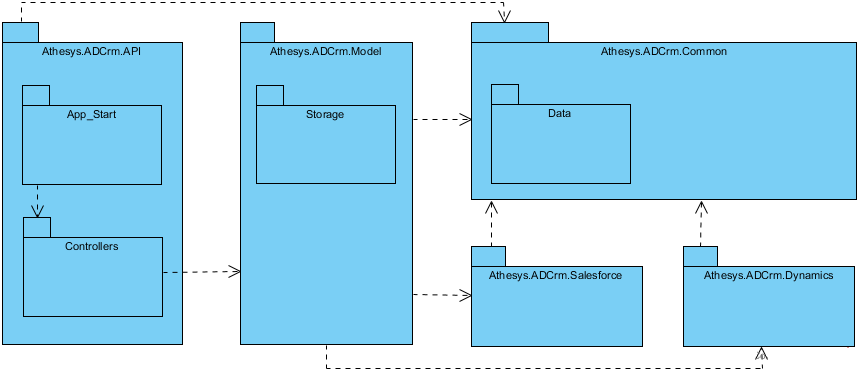
\includegraphics[width=\linewidth]{images/modulesDiagram}
%	\caption{Diagramma dei moduli di ADCrm}
%	\label{fig:generalUMLDiagram}
%\end{figure}

\begin{figure}[H]
	\centering
	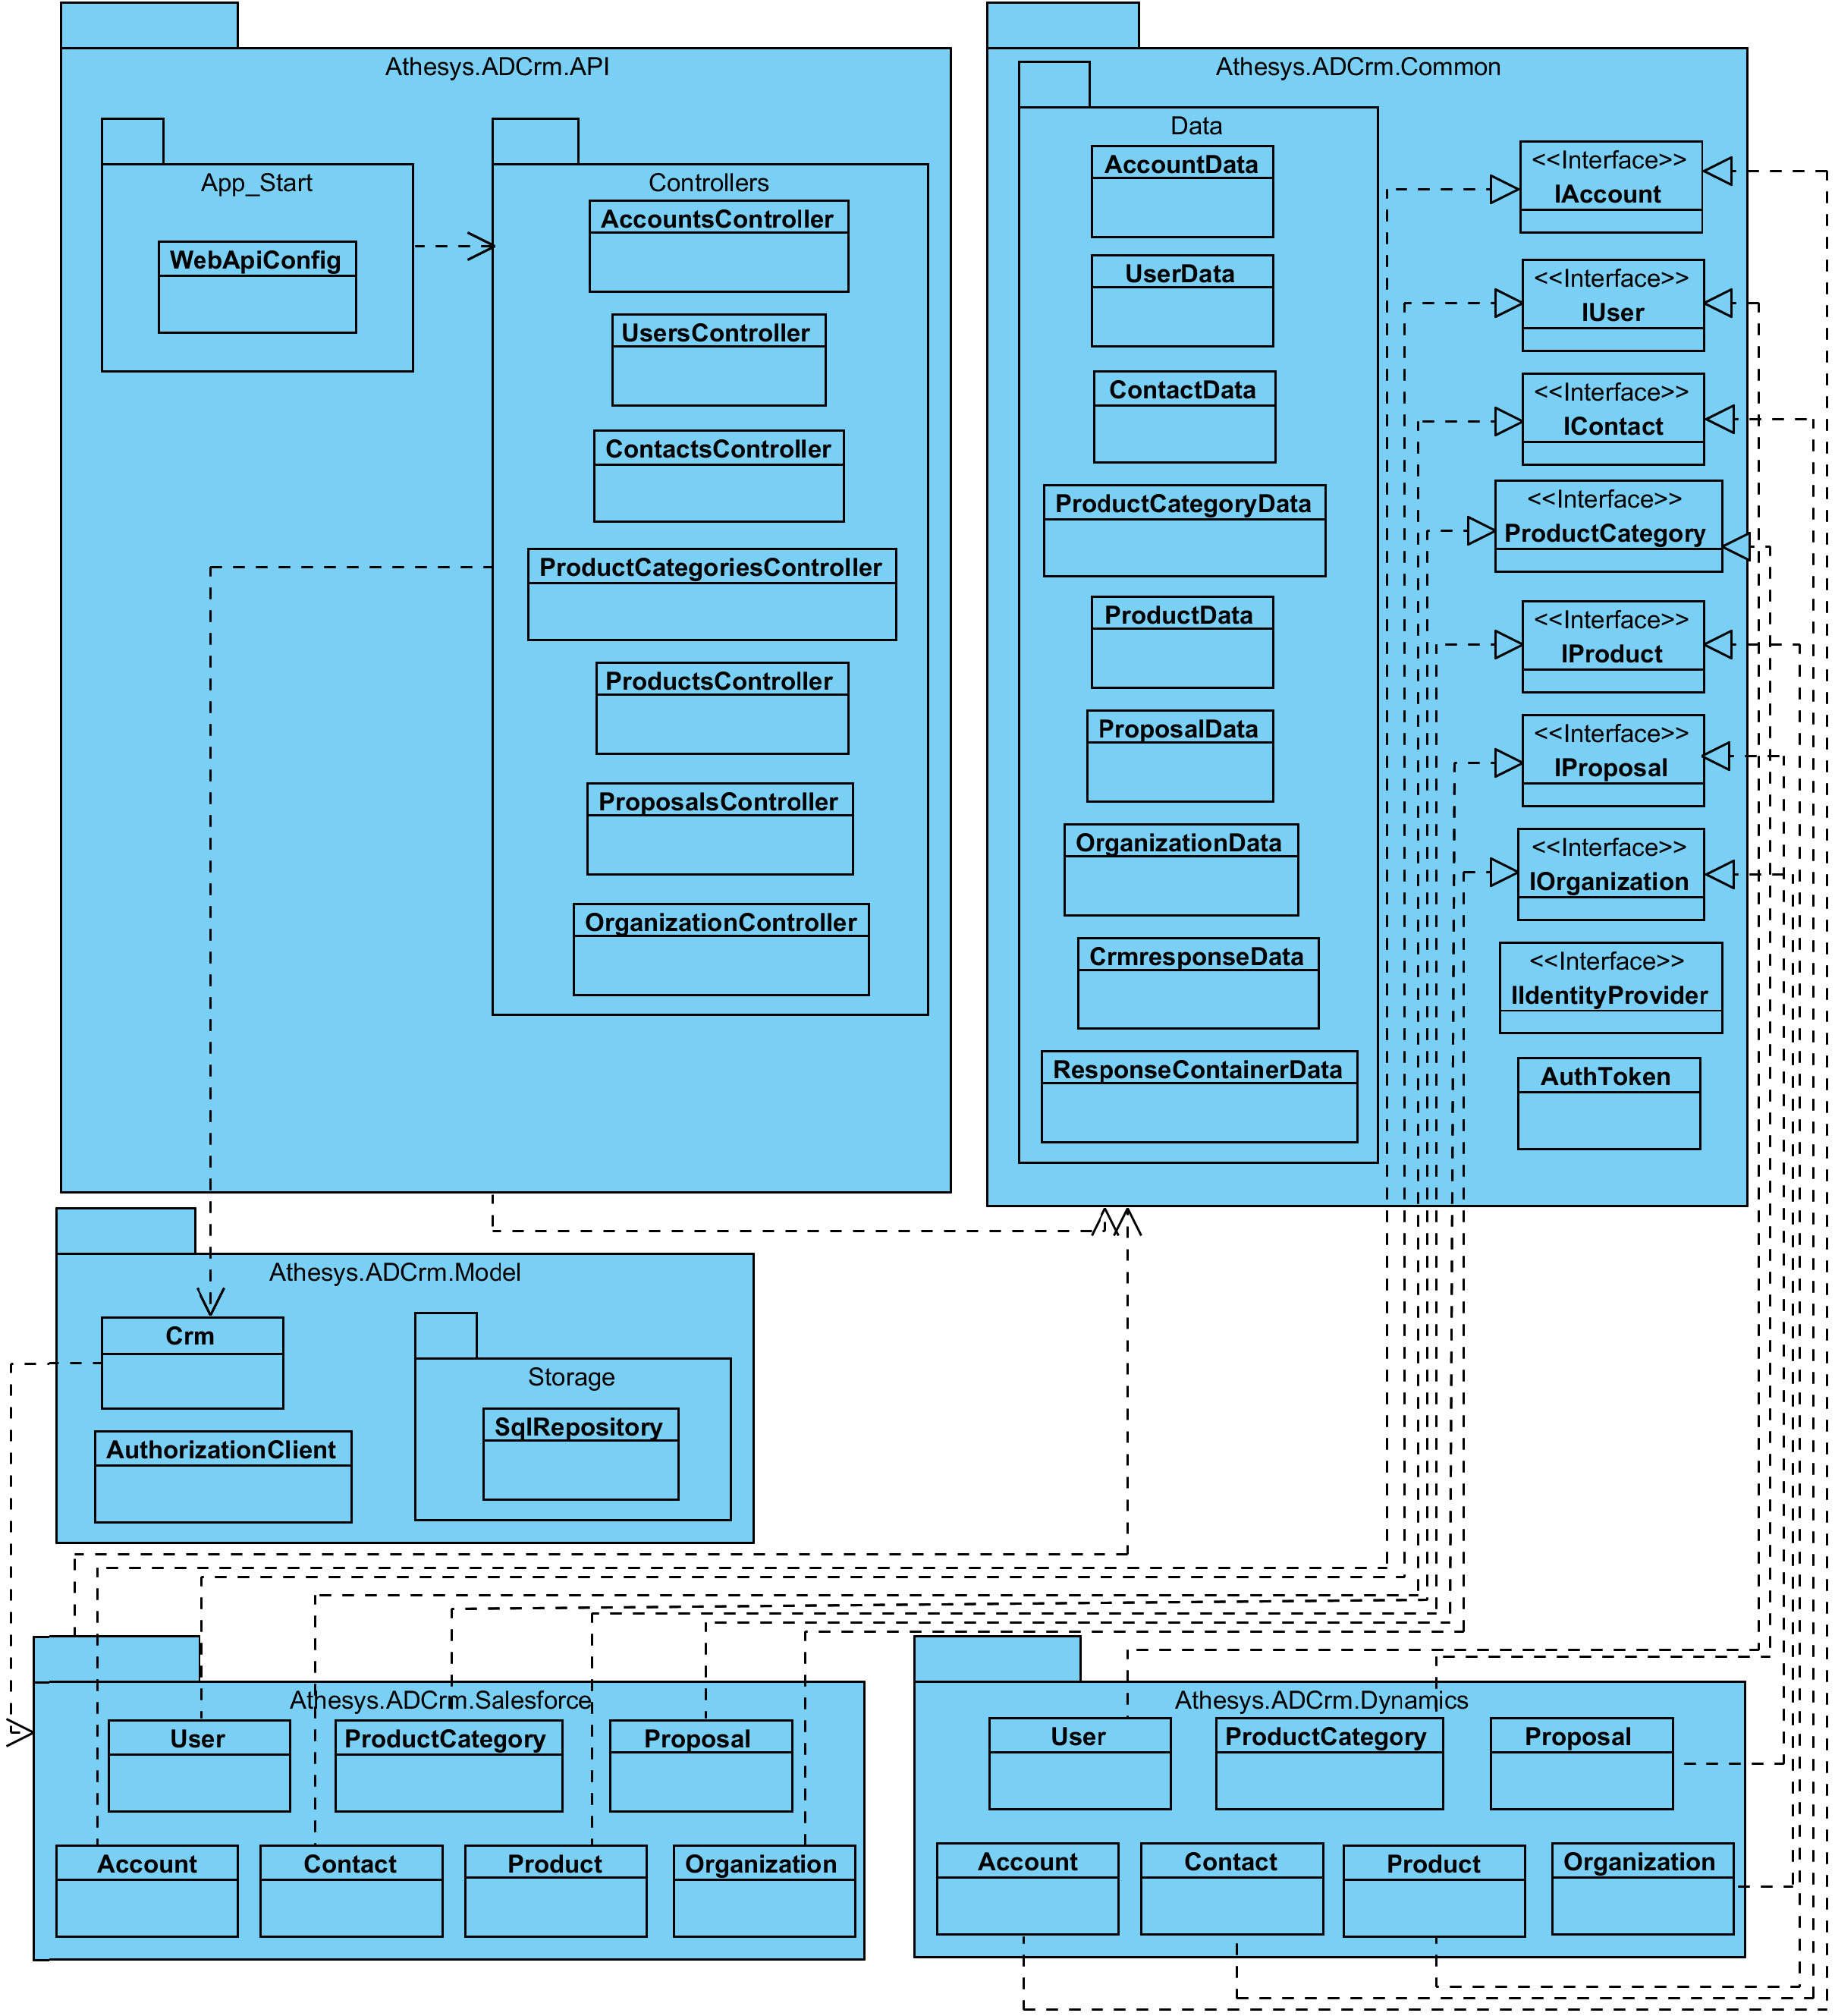
\includegraphics[width=\linewidth]{images/general2}
	\caption{Diagramma UML di ADCrm}
	\label{fig:modulesdiagram}
\end{figure}



\subsection{Athesys.ADCrm.API}
\begin{figure}[H]
	\centering
	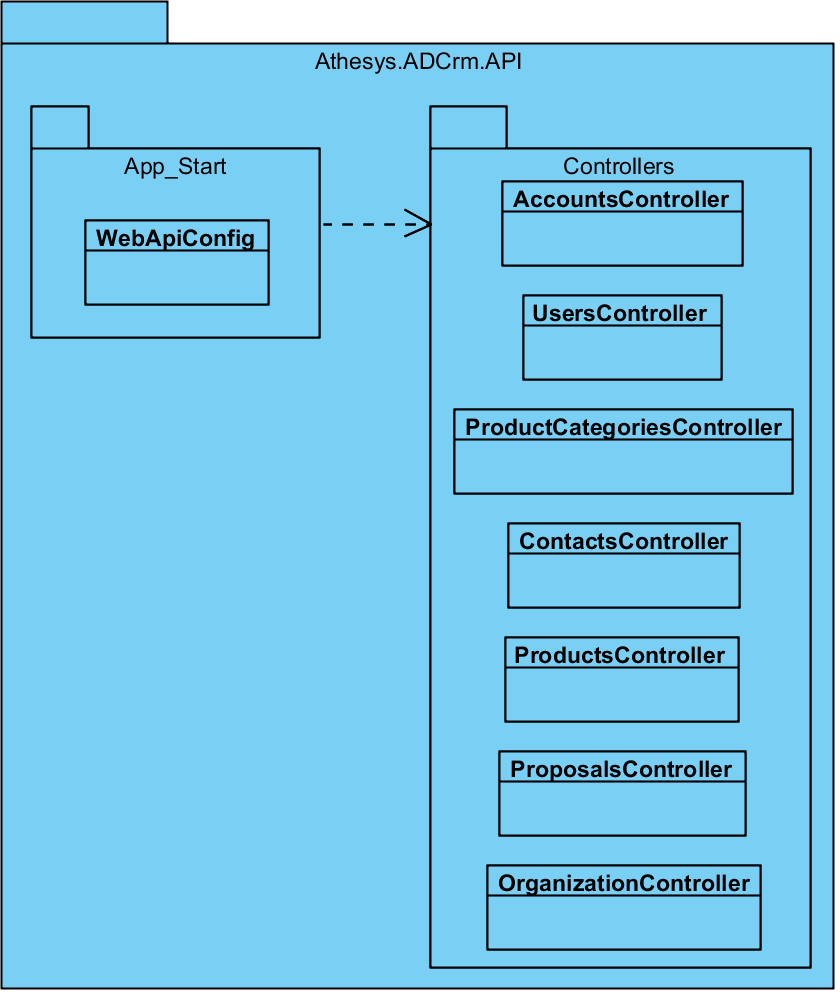
\includegraphics[width=\linewidth]{images/modules/API}
	\caption{Diagramma UML del package Athesys.ADCrm.API}
	\label{fig:api}
\end{figure}
\paragraph{Descrizione:} 
Questo \glo{package} è utilizzato per esporre le API REST all'applicazione web ADProject. In esso vengono definite le \glo{route} che è possibile chiamare, ad ognuna di esse viene associato un metodo di un particolare controller. 





\subsection{Athesys.ADCrm.API.AppStart}
\paragraph{Descrizione:} 
Questo \glo{package} contiene la classe che si occupa di definire le \glo{route} che verranno esposte dall'applicazione.

\subsection{Athesys.ADCrm.API.Controllers}
\begin{figure}[H]
	\centering
	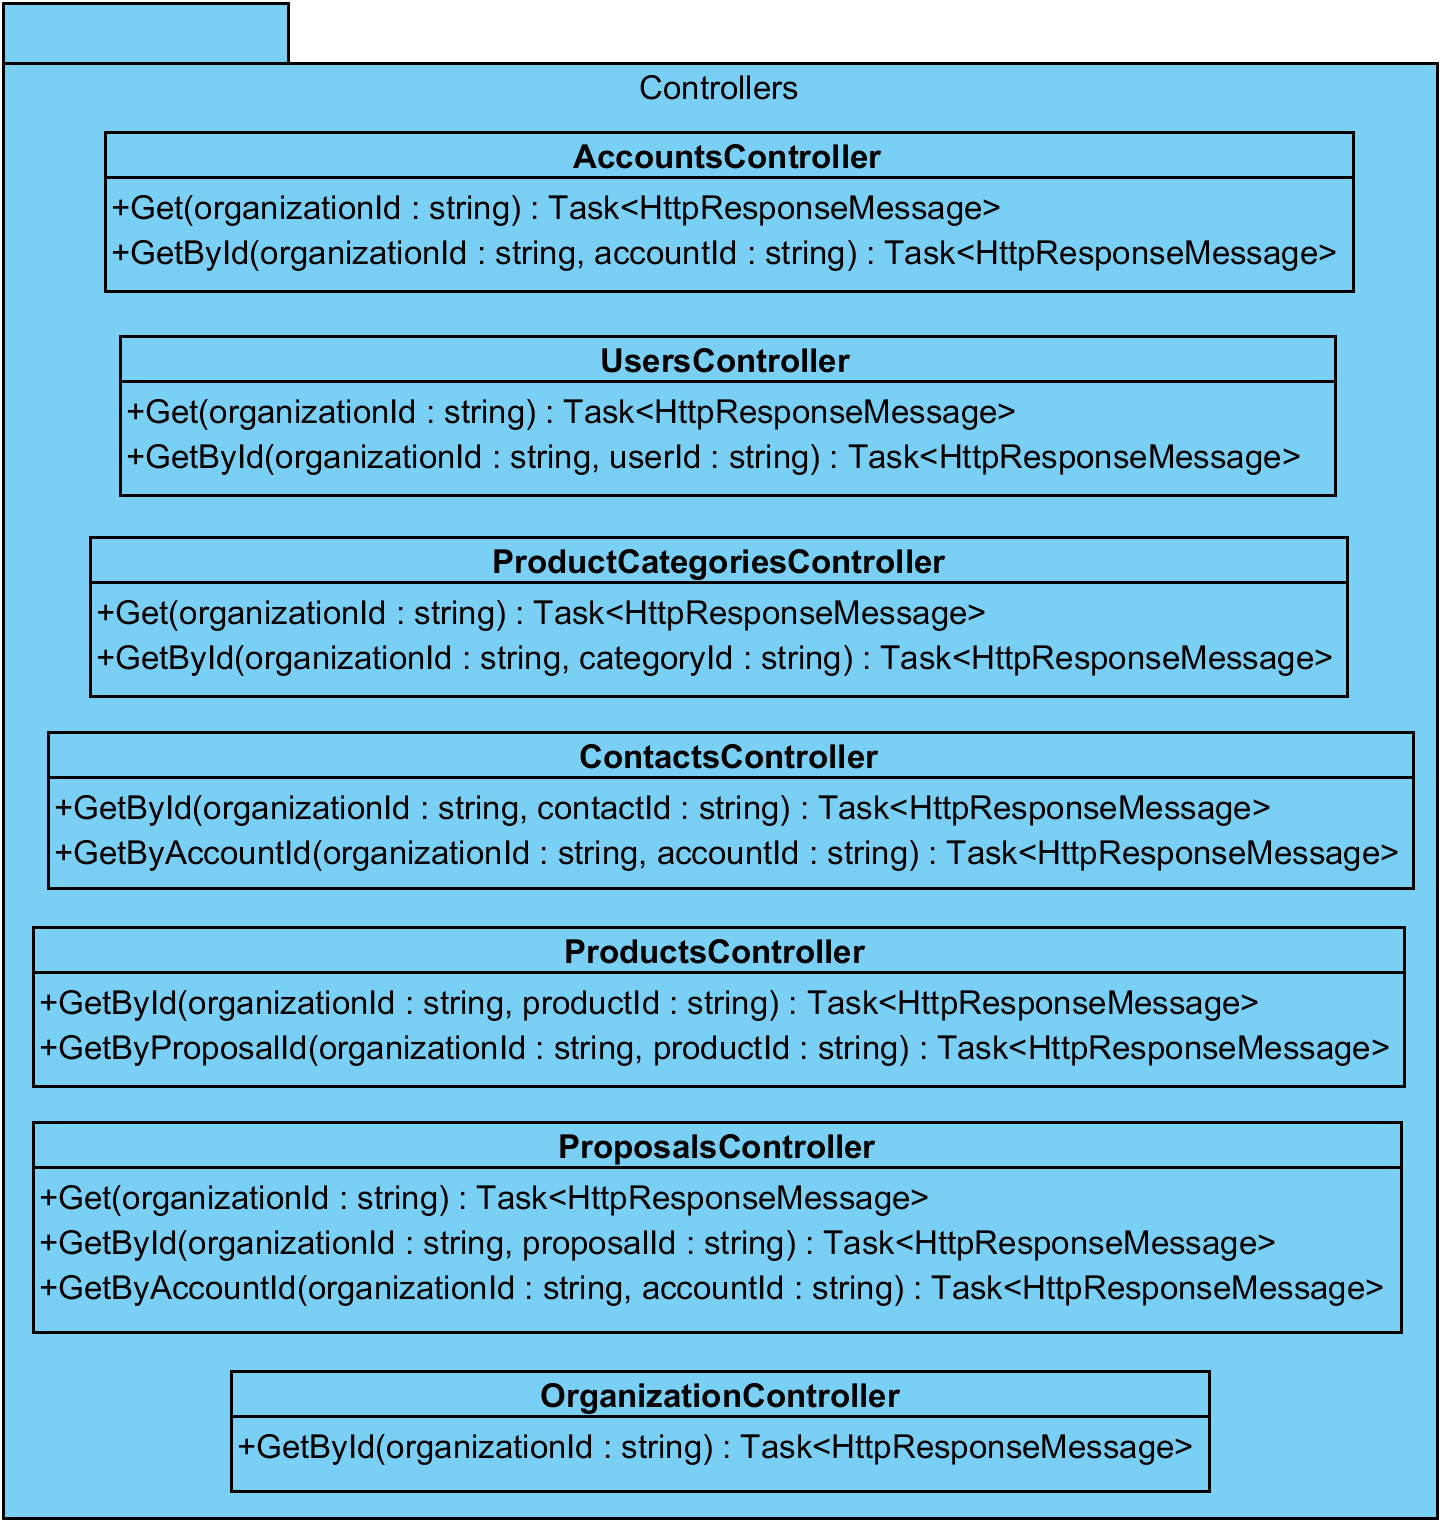
\includegraphics[width=\linewidth]{images/modules/Controllers}
	\caption{Diagramma UML del package Athesys.ADCrm.API::Controllers}
	\label{fig:controllers}
\end{figure}
\paragraph{Descrizione:} Questo \glo{package} contiene tutte le classi controller contenenti i metodi necessari a rispondere alle richieste http effettuate alle \glo{route}.


\subsubsection{AccountsController (class)}
\paragraph{Descrizione:}
Classe che serve per gestire le chiamate http richiedenti dati relativi all'entità Account. Utilizzando la classe Athesys.ADCrm.Model::Crm (che implementa il design pattern Factory) vengono creati oggetti sui quali si possono invocare metodi per interrogare le API di uno specifico CRM.
I dati recuperati vengono incapsulati in una risposta http e ritornati ad ADProject.

\paragraph{Metodi:}\hfill
\begin{itemize}
	\itemsep0em 
	\item 
		\begin{lstlisting}
		Public async Task<HttpResponseMessage> Get(organizationId : string)
		\end{lstlisting}
		Metodo invocato quando viene inviata una richiesta http GET alla route "api/organization/{organizationId}/accounts", ritornado una risposta http contenente la lista di tutti gli Account censiti nel CRM.\\
		\textbf{\small Argomenti:}
		\begin{enumerate}[leftmargin=*]
			\itemsep0em 
			\item \begin{lstlisting}
			organizationId : string 
			\end{lstlisting}
			Rapprensenta l'identificativo univoco legato all'utenza aziendale con cui accedere al servizio CRM
		\end{enumerate}
		
	\item 
		\begin{lstlisting}
		Public async Task<HttpResponseMessage> GetById(organizationId : string, accountId : string)
		\end{lstlisting}
		Metodo invocato quando viene inviata una richiesta http GET alla route "api/organization/{organizationId}/accounts/{accountId}", ritornando una risposta http contenente l'Account avente id = {accountId}.\\
		\textbf{\small Argomenti:}
		\begin{enumerate}[leftmargin=*]
			\itemsep0em 
			\item 
				\begin{lstlisting}
				organizationId : string 
				\end{lstlisting}
				Rappresenta l'identificativo univoco legato all'utenza aziendale con cui accedere al servizio CRM
			\item 
				\begin{lstlisting}
				accountId : string
				\end{lstlisting}
				Rappresenta l'identificativo univoco legato ad un Account del CRM, attraverso il quale si andrà a richiedere i dati voluti
		\end{enumerate}
\end{itemize}

\subsubsection{ProposalsController (class)}

\paragraph{Descrizione:}
Classe che serve per gestire le chiamate http richiedenti dati relativi all'entità Proposal. Utilizzando la classe Athesys.ADCrm.Model::Crm (che implementa il design pattern Factory) vengono creati oggetti sui quali si possono invocare metodi per interrogare le API di uno specifico CRM. I dati recuperati vengono incapsulati in una risposta http e ritornati ad ADProject.

\paragraph{Metodi:}\hfill
\begin{itemize}
	\itemsep0em 
	\item 
	\begin{lstlisting}
	Public async Task<HttpResponseMessage> Get(organizationId : string)
	\end{lstlisting}
	Metodo invocato quando viene inviata una richiesta http GET alla route "api/organization/{organizationId}/proposals", ritornando una risposta http contenente tutte le offerte commerciali censite nel CRM.\\
	\textbf{\small Argomenti:}
	\begin{enumerate}[leftmargin=*]
		\itemsep0em 
		\item \begin{lstlisting}
		organizationId : string 
		\end{lstlisting}
		Rappresenta l'identificativo univoco legato all'utenza aziendale con cui accedere al servizio CRM.
	\end{enumerate}
	
	\item 
	\begin{lstlisting}
	Public async Task<HttpResponseMessage> GetById(organizationId : string,  proposalId : string)
	\end{lstlisting}
	Metodo invocato quando viene inviata una richiesta http GET alla route "api/organization/{organizationId}/proposals/{proposalId}", ritornando una risposta http contenente l'offerta commerciale avente id = {proposalId}.\\
	\textbf{\small Argomenti:}
	\begin{enumerate}[leftmargin=*]
		\itemsep0em 
		\item 
		\begin{lstlisting}
		organizationId : string 
		\end{lstlisting}
		Rapprensenta l'identificativo univoco legato all'utenza aziendale con cui accedere al servizio CRM;
		\item 
		\begin{lstlisting}
		proposalId : string
		\end{lstlisting}
		Rappresenta l'identificativo univoco legato ad un offerta commerciale del CRM, attraverso il quale si andrà a richiedere i dati voluti.
	\end{enumerate}

	\item 
	\begin{lstlisting}
	Public async Task<HttpResponseMessage> GetByAccountId(organizationId : string,  accountId : string)
	\end{lstlisting}
	Metodo invocato quando viene inviata una richiesta http GET alla route "api/organization/{organizationId}/accounts/{accountId}/proposals", ritornando una risposta http contenente la lista delle proposte legate all'account avente id = {proposalId}.\\
	\textbf{\small Argomenti:}
	\begin{enumerate}[leftmargin=*]
		\itemsep0em 
		\item 
		\begin{lstlisting}
		organizationId : string 
		\end{lstlisting}
		Rapprensenta l'identificativo univoco legato all'utenza aziendale con cui accedere al servizio CRM;
		\item 
		\begin{lstlisting}
		accountId : string
		\end{lstlisting}
		Rappresenta l'identificativo univoco legato all'account di un azienda cliente CRM, attraverso il quale si andrà a richiedere i dati voluti.
	\end{enumerate}
\end{itemize}

\vfill
\subsection{Athesys.ADCrm.Common}

	\begin{figure}[H]
		\centering
		\rotatebox{90}{\includegraphics[width=.89\textheight,height=1.08\linewidth]{images/modules/common}}
		
		\caption{Diagramma UML del package Athesys.ADCrm.Common}
		\label{fig:common}
	\end{figure}


\newpage
\paragraph{Descrizione:}
Questo \glo{package} contiene il \glo{package} Data(avente le classi DTO) e tutte le interfacce che dovranno essere implementate diversamente per ogni CRM che si vuole collegare all'applicazione. 
%TODO: da modificare la descrizione

\subsubsection{IIdentityProvider (interface)}

\paragraph{Descrizione:}
Interfaccia che dovrà essere implementata dalle classi concrete Athesys.ADCrm.Salesforce::IdentityProvider e\\ Athesys.ADCrm.Dynamics::IdentityProvider, essa definisce i metodi utilizzati per ottenere i \glo{token} di autenticazione e di refresh dai CRM, ed inoltre espone il metodo per effettuare inviare le \glo{query} di recupero dei dati.

\paragraph{Metodi:}\hfill
\begin{itemize}
	\itemsep0em 	
	\item 
	\begin{lstlisting}
	 Task<AuthToken> GetAuthTokenAsync(string authorizationCode, string clientId, string clientSecret, string redirectUrl)
	\end{lstlisting}
	Metodo da implementare per ottenere i \glo{token} da aggiungere all'\glo{header} delle richieste http per poter effettuare le query al CRM e il \glo{token} di refresh per otterene nuovi \glo{token} una volta scaduti. Tutti i paramentri passati al metodo sono essenziali per effettuare la suddetta richiesta.\\
	\textbf{\small Argomenti:}
	\begin{enumerate}[leftmargin=*]
		\itemsep0em 
		\item 
		\begin{lstlisting}
		authorizationCode : string
		\end{lstlisting}
		E' un codice che viene generato nel caso l'utente abbia inserito le credenziali d'accesso al CRM;
		%TODO: da aggiungere i riferimenti alla sezione;
		\item 
		\begin{lstlisting}
		clientSecret : string
		\end{lstlisting}
		E' un codice alfanumerico identificativo dell'applicazione, che non cambia nel tempo, generato dall'CRM. Esso è fondamentale per permettere il collegamento OAuth all'applicazione; 
		%TODO: in caso da modificare questa parte
		\item 
		\begin{lstlisting}
		clientId : string
		\end{lstlisting}
		E' un codice alfanumerico che non cambia nel tempo, generato dall'CRM. Esso è fondamentale per permettere il collegamento \glo{OAuth} all'applicazione. 
		%TODO: in caso da modificare questa parte
		\item 
		\begin{lstlisting}
		redirectUrl : string
		\end{lstlisting}
		E' l'url su cui si vuole far arrivare le risposte del CRM.
		%TODO: in caso da modificare questa parte
	\end{enumerate}
	
	\item 
	\begin{lstlisting}
	Task<string> RenewAuthTokenAsync(string refreshToken, string clientId, string clientSecret)
	\end{lstlisting}
	Metodo da implementare per ottenere un nuovo \glo{token} di autorizzazione nel caso il precedente sia scaduto.\\
	\textbf{\small Argomenti:}
	\begin{enumerate}[leftmargin=*]
		\itemsep0em
		\item 
		\begin{lstlisting}
		refreshToken : string
		\end{lstlisting}
		E' un codice generato dall'CRM fornito una volta effettuato l'accesso con \glo{OAuth}. Questo permette di ottenere nuovi \glo{token} di autorizzazione senza dover effettuare nuovamente la procedura di login;
		\item 
		\begin{lstlisting}
		clientId : string
		\end{lstlisting}
		E' un codice alfanumerico che non cambia nel tempo, generato dall'CRM. Esso è fondamentale per permettere il collegamento OAuth all'applicazione. 
		%TODO: in caso da modificare questa parte
		\item 
		\begin{lstlisting}
		clientSecret : string
		\end{lstlisting}
		E' un codice alfanumerico identificativo dell'applicazione, che non cambia nel tempo, generato dall'CRM. Esso è fondamentale per permettere il collegamento OAuth all'applicazione; 
		%TODO: in caso da modificare questa parte
	\end{enumerate}

	\item 
	\begin{lstlisting}
	 public async Task<QueryResponse> SendQueryWithRefresh(string resourceProvider,string accessToken,string refreshToken,string clientId, string clientSecret, Action<HttpRequestMessage> addQuryAction)
	\end{lstlisting}
	Metodo da implementare per inviare la richiesta http con la \glo{query} per ottenere i dati desiderati dal CRM. Nel caso il \glo{token} d'autorizzazione passato fosse scaduto il metodo si occupa di recuperarne uno nuovo tramite la procedura di refresh. Nella successiva descrizione degli argomenti, per evitare inutili ripetizioni, vengono esclusi quelli già descritti nei sopracitati metodi.\\
	\textbf{\small Argomenti:}
	\begin{enumerate}[leftmargin=*]
		\itemsep0em
		\item 
		\begin{lstlisting}
		resourceProvider : string
		\end{lstlisting}
		E' l'uri a cui si devono effettuare le \glo{query};
		\item 
		\begin{lstlisting}
		addQuryAction : Action<HttpRequestMessage>
		\end{lstlisting}
		E' il corpo della \glo{query} in formato di HttpRequestMessage. 
		%TODO: in caso da modificare questa parte
	\end{enumerate}
\end{itemize}

\subsubsection{IProposal (interface)}

\paragraph{Descrizione:}
Interfaccia che dovrà essere implementata dalle classi concrete Athesys.ADCrm.Salesforce::Proposal e\\ Athesys.ADCrm.Dynamics::Proposal, essa definisce i metodi utilizzati per interrogare i rispettivi CRM attraverso le API REST esposte, restituendo la risposta http incapsulata all'interno di un DTO di tipo ResponseContainerData.

\paragraph{Metodi:}\hfill
\begin{itemize}
	\itemsep0em 
	\item 
	\begin{lstlisting}
	Task<ResponseContainerData<ProposalData>> GetAll()
	\end{lstlisting}
	Metodo da implementare per interrogare il CRM ritornando la lista di tutte le offerte commerciali censite nello stesso. Il metodo restituisce il DTO ResponseContainerData istanziato al tipo ProposalData essendo una classe \glo{generic}.\\
	
	\item 
	\begin{lstlisting}
	Task<ResponseContainerData<ProposalData>> GetById(proposalId : string)
	\end{lstlisting}
	Metodo da implementare per interrogare il CRM ritornando l'offerta commerciale avente id = {proposalId}. Il metodo restituisce il DTO ResponseContainerData istanziato al tipo ProposalData essendo una classe \glo{generic}.\\
	\textbf{\small Argomenti:}
	\begin{enumerate}[leftmargin=*]
		\itemsep0em 
		\item 
		\begin{lstlisting}
		proposalId : string
		\end{lstlisting}
		Rappresenta l'identificativo univoco legato ad un offerta commerciale del CRM, attraverso il quale si andrà a richiedere i dati voluti.
	\end{enumerate}
	
	\item 
	\begin{lstlisting}
	Task<ResponseContainerData<ProposalData>> GetByAccountId(accountId : string)
	\end{lstlisting}
	Metodo da implementare per interrogare il CRM ritornando la lista di tutte le offerte commerciali legate all'account avente id = {accountId}. Il metodo restituisce il DTO ResponseContainerData istanziato al tipo ProposalData essendo una classe \glo{generic}.\\
	\textbf{\small Argomenti:}
	\begin{enumerate}[leftmargin=*]
		\itemsep0em
		\item 
		\begin{lstlisting}
		accountId : string
		\end{lstlisting}
		Rappresenta l'identificativo univoco legato all'account di un azienda cliente CRM, attraverso il quale si andrà a richiedere i dati voluti.
	\end{enumerate}
\end{itemize}

\subsection{Athesys.ADCrm.API.Data}
\begin{figure}[H]
	\centering
	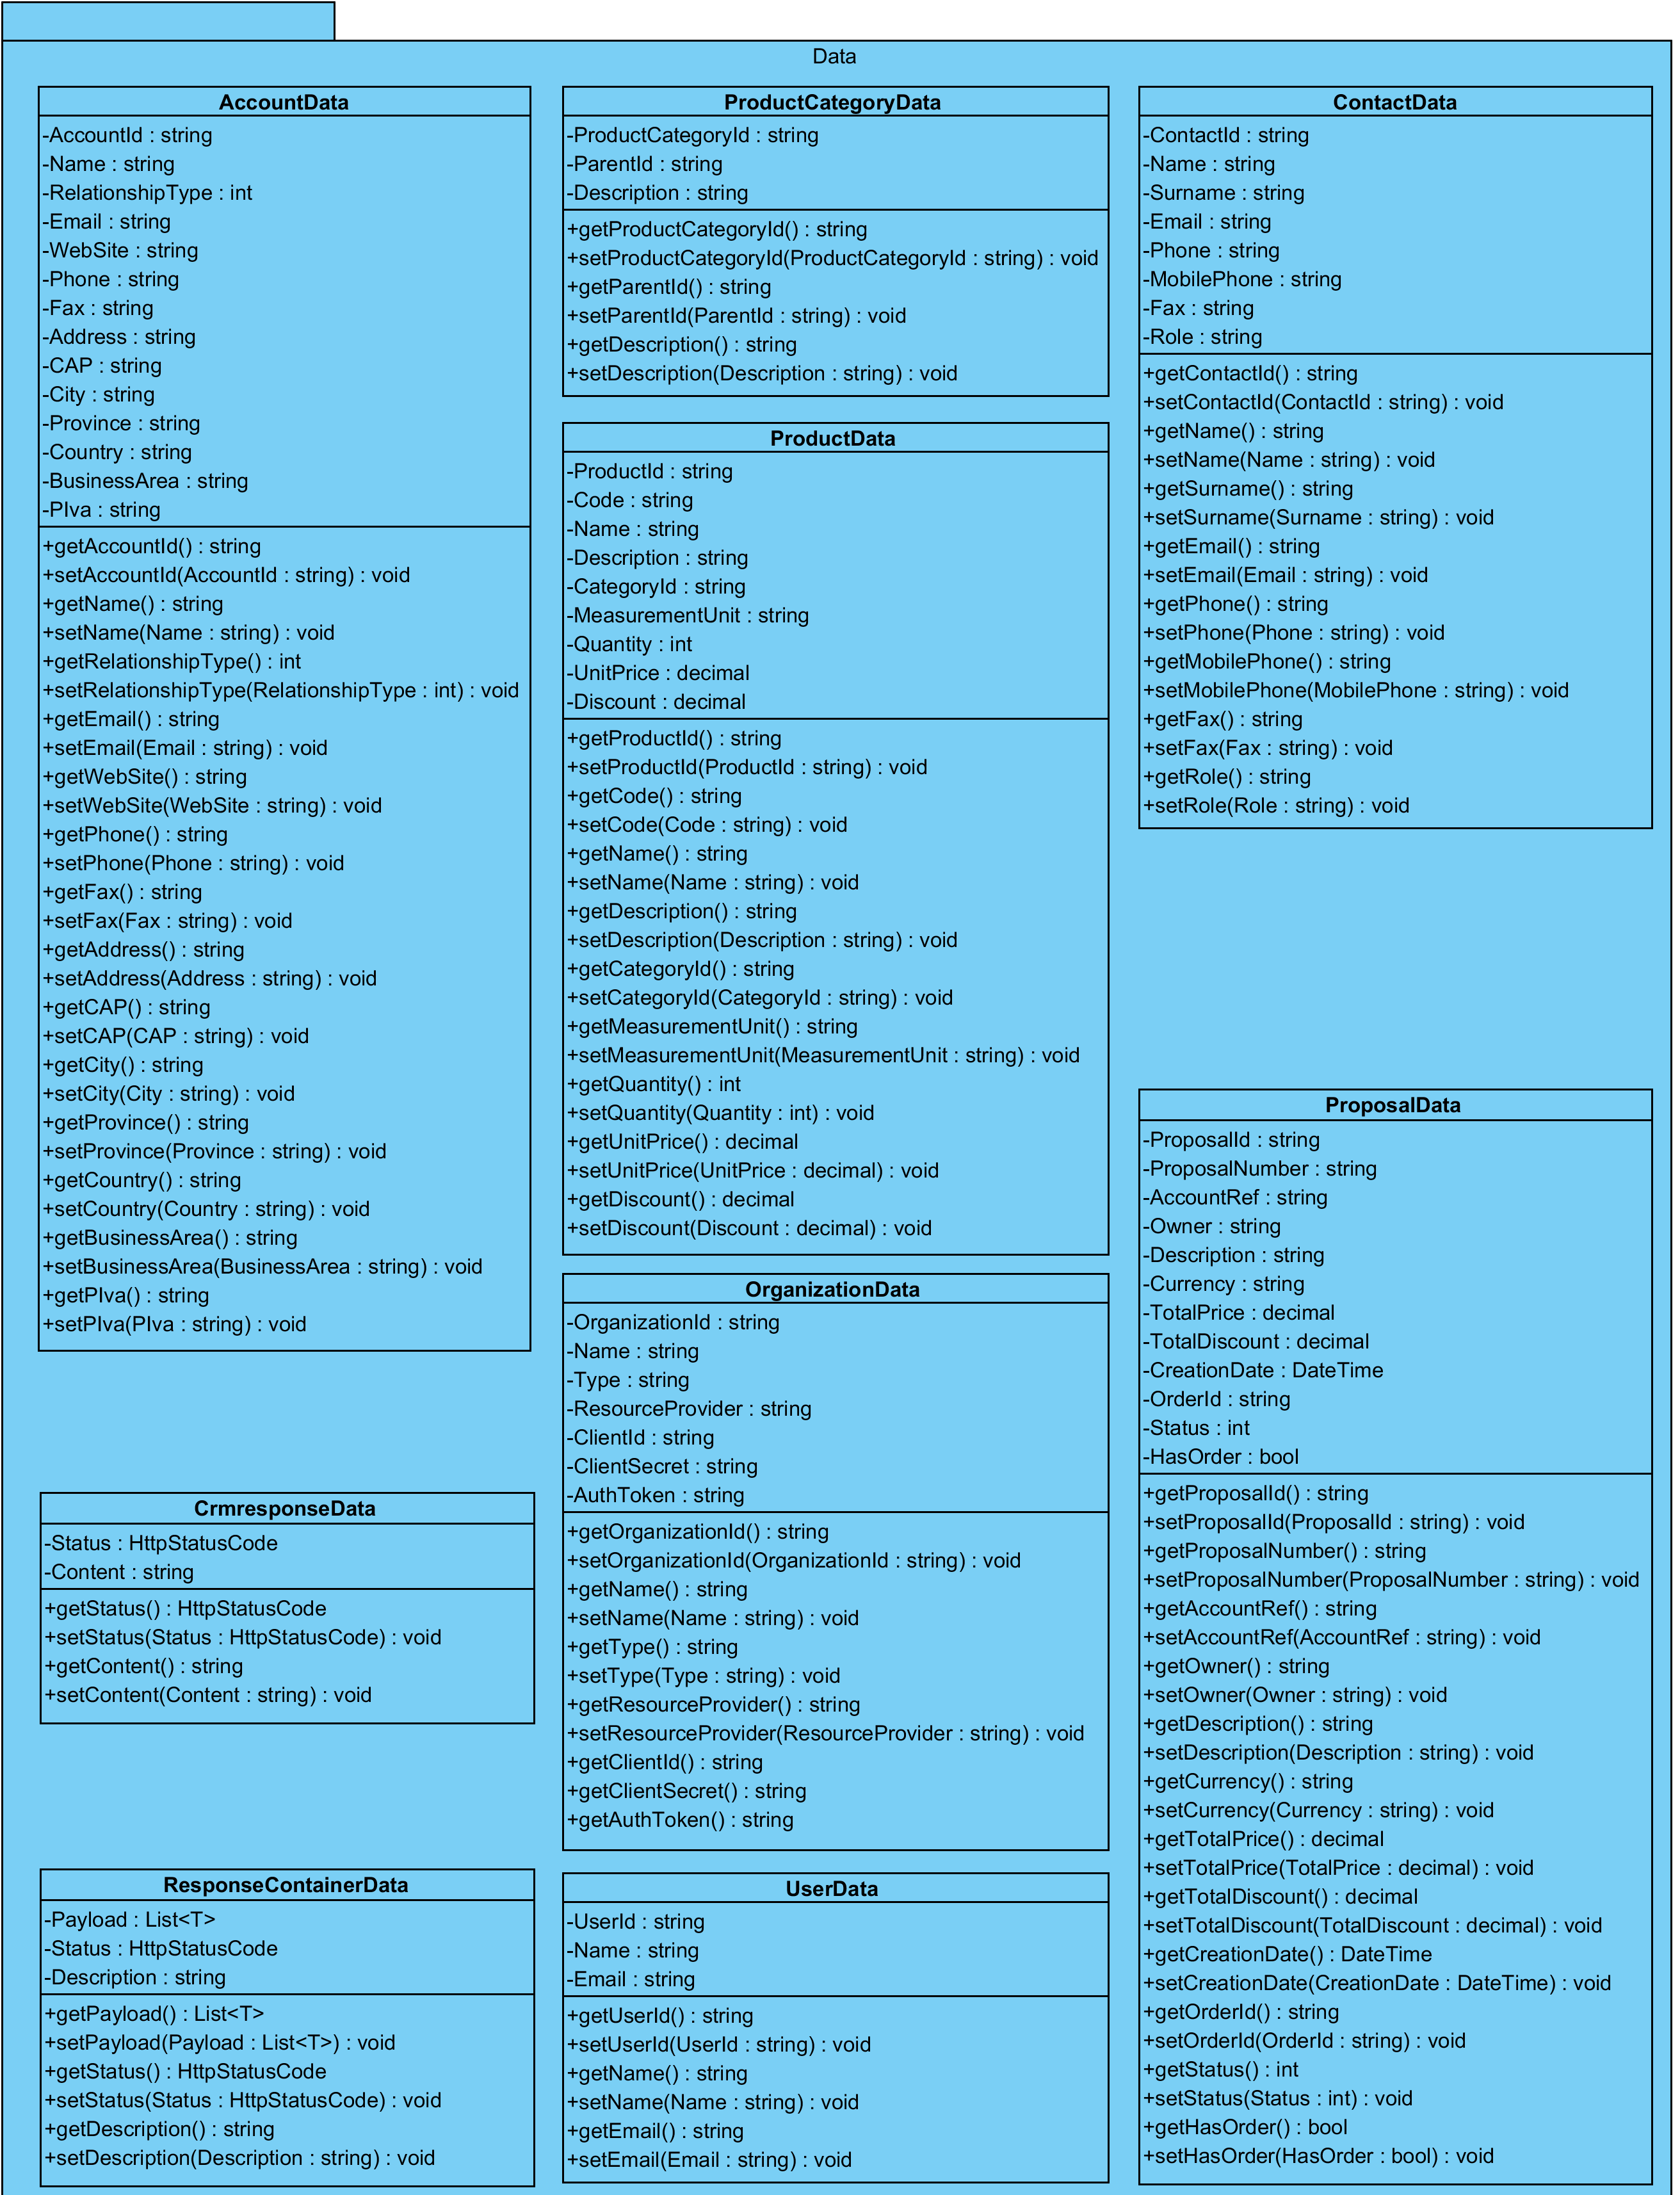
\includegraphics[width=\linewidth]{images/modules/Data}
	\caption{Diagramma UML del package Athesys.ADCrm.Common::Data}
	\label{fig:data}
\end{figure}
\paragraph{Description:}
Questo \glo{package} contiene tutti i vari DTO definiti per ogni entità di dati che si vuole restituire alle chiamate effettuate da ADProject ed inoltre quelle necessarie per gestire le risposte le risposte provenienti dai CRM. 
Segue in questa sezione una breve descrizione delle classi principali, sorvolando sui metodi delle stesse in quanto sono tutti \glo{accessors} \glo{getter} e \glo{setter}.


\subsubsection{ProposalData (class)}
\paragraph{Descrizione:}
Classe che rappresenta un oggetto DTO per modellare l'entità \textit{Proposal}.
In essa sono presenti i metodi \glo{getter} e \glo{setter} e tutti i campi dati (privati) contenenti gli elementi che caratterizzano un offerta commerciale, quali: l'identificativo univoco della stessa, il cliente a cui è stata proposta, il costo totale, un eventuale sconto e molti altri dati.
Gli oggetti di questa classe, contenente i dati provenienti dal CRM, verranno incapsulati all'interno della risposta http restituita ad ADProject.

\subsubsection{CrmResponseData (class)}
\paragraph{Descrizione:}
Classe che rappresenta un oggetto DTO per modellare le risposte http provenienti dal CRM.
Questa classe ha solamente due campi dati (ed i relativi \glo{accessors}):
\begin{itemize}
	\item 	
	\begin{lstlisting}
	Private HttpStatusCode Status
	\end{lstlisting}
	In questo campo dati viene salvato il codice di stato http della risposta mandata dal CRM;
	\item
	\begin{lstlisting}
	Private string Content
	\end{lstlisting}
	In questo campo dati viene salvato il \glo{Json} della risposta mandata dal CRM.
\end{itemize}

\subsubsection{ResponseContainerData (class)}
\paragraph{Descrizione:}
Classe che rappresenta un oggetto DTO per modellare le risposte http da inviare a ADProject.
Questa classe ha tre campi dati (ed i relativi \glo{accessors}):
\begin{itemize}
	\item 	
	\begin{lstlisting}
	private List<T> Payload
	\end{lstlisting}
	In questo campo dati è una lista di \glo{generics} che viene istanziata al tipo di uno degli oggetti DTO di questo \glo{package} (AccountData,ProposalData,ProductData,ContactData,UserData,ProductCategoryData o OrganizationData);
	
	\item 	
	\begin{lstlisting}
	private HttpStatusCode Status
	\end{lstlisting}
	In questo campo dati viene salvato il codice di stato http che dovrà assumere la risposta da inviare ad ADProject;
	
	\item
	\begin{lstlisting}
	private string Description
	\end{lstlisting}
	In questo campo dati, in caso di errore, viene aggiunta una breve descrizione testuale dello stesso.
\end{itemize}




\subsection{Athesys.ADCrm.Model}
Questo \glo{package} contiene tutte le classi concrete in comune tra i CRM che si vogliono collegare all'applicazione.
La classe principale del \glo{package} è Athesys.ADCrm.Model::Crm.
\subsubsection{Crm (class)}
\paragraph{Descrizione:}
Questa classe implementa il design pattern Factory ed è usata dai controllers per produrre oggetti concreti di un particolare CRM (su cui invocare i metodi per recuperare i dati dallo stesso) senza conoscere a priori il tipo di CRM richiesto (Dynamics o SalesForce).

\begin{figure}[H]
	\centering
	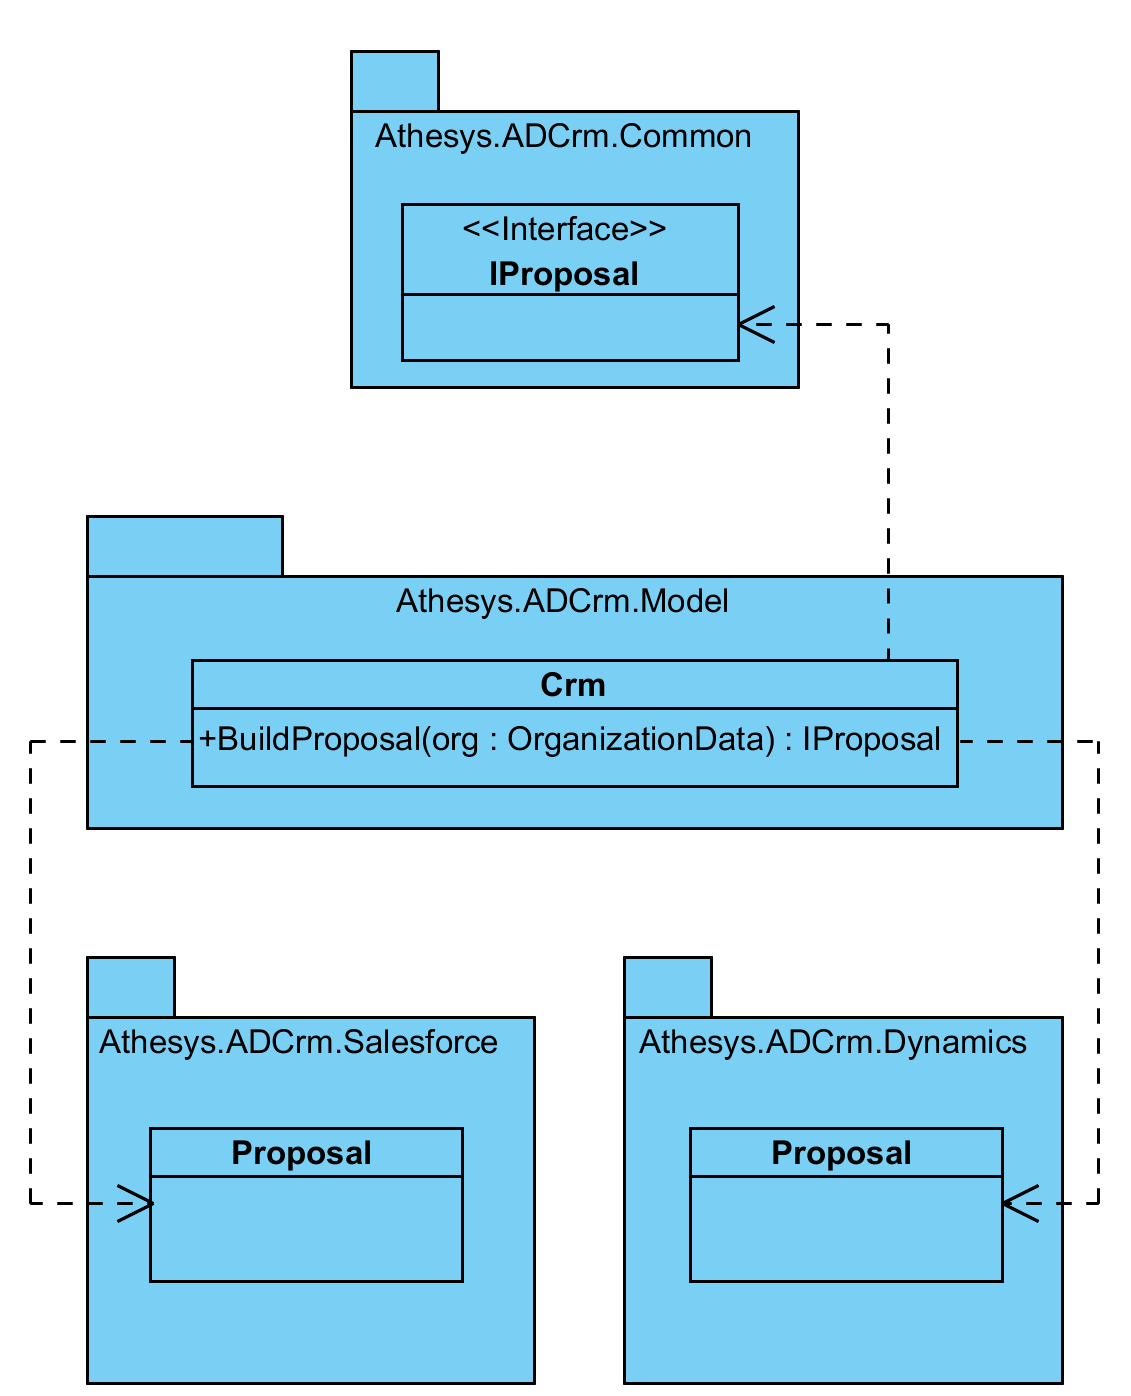
\includegraphics[width=\linewidth]{images/factoryInADCrm}
	\caption{Diagramma semplificato del pattern Factory per ADCrm}
	\label{fig:factoryInADCrm}
\end{figure}
Di seguito vengono riportati alcuni metodi significativi della classe per esemplificarne il funzionamento generale.


\paragraph{Metodi:}\hfill
\begin{itemize}
	\itemsep0em 
	\item 
	\begin{lstlisting}
	  public static async Task<OrganizationData> BuildOrganization(string organizationId)	
	\end{lstlisting}
	Metodo che costruisce un oggetto di tipo OrganizationData, appartenente ad un particolare CRM, in base alla tipologia del parametro passato.
	Tutti i campi dati dell'oggetto ritornato vengono impostati dal database dell'applicazione che contiene i parametri di connessione ai vari CRM.
	\\
	\textbf{\small Argomenti:}
	\begin{enumerate}[leftmargin=*]
		\itemsep0em 
		\item 
		\begin{lstlisting}
		organizationId : string
		\end{lstlisting}
		Rappresenta la tipologia di CRM a cui ci si deve collegare. Questo dati si ottiene grazie alle route definite nella sezione \ref{apiRest} (eg. api/organization/\{\textbf{organizationId}\}/accounts).
	\end{enumerate}
	
	\item 
	\begin{lstlisting}
     public static IProposal BuildProposal(OrganizationData org)
	\end{lstlisting}
	Metodo che, in base alla tipologia di organizzazione passata per parametro, costruisce un oggetto Proposal per un particolare tipo di CRM\\
	\textbf{\small Argomenti:}
	\begin{enumerate}[leftmargin=*]
		\itemsep0em
		\item 
		\begin{lstlisting}
		org : OrganizationData
		\end{lstlisting}
		Rappresenta la tipologia di CRM da cui si vogliono recuperare le proposte commerciali.
	\end{enumerate}
\end{itemize}
 
\subsection{Athesys.ADCrm.Salesforce}
Questo \glo{package} contiene tutte le classi che implementano le interfacce definite in Athesys.ADCrm.Common e, sviluppando  restituiscono ai controllers di Athesys.ADCrm.API i vari oggetti DTO delle entità del \glo{package} Athesys.ADCrm.Common.Data.
Di seguito vengono descritte brevemente le uniche tre classi che hanno un comportamento diverso da quanto sopracitato.

\subsubsection{ResponceMapper (class)}
\paragraph{Descrizione:}
Questa classe ha la funzione di mappare le risposte provenienti dal CRM modificandole in base alle esigenze di ADProject.
Per esempio se dal CRM arrivasse una risposta d'errore con codice di stato http 500 (quindi un errore interno del server), non si dovrà restituire ad ADProject una risposta lo stesso codice di stato, in quanto verrebbe interpretato come un errore del servizio e non del CRM. C'è quindi l'esigenza di modificare ad-hoc le risposte per renderle fruibili dal richiedente delle stesse.
%TODO: controllare questa parte

\subsection{Athesys.ADCrm.Dynamics}
Questo \glo{package} contiene tutte le classi che implementano le interfacce definite in Athesys.ADCrm.Common e restituiscono ai controller di Athesys.ADCrm.API i vari oggetti DTO di tipo Athesys.ADCrm.Common.Data al fine di incapsularli nella risposta http.
Viene omessa la descrizione delle classi e dei metodi in quanto risulta identica a quella del \glo{package} \textit{Athesys.ADCrm.Salesforce}

\subsection{Database}
Il database è utilizzato per salvare i dati necessari a collegarsi per effettuare l'accesso e le richieste ai CRM, vista la bassissima mole di dati da salvare si è deciso di optare per un semplicissimo database \glo{SQL} composto da una singola tabella, di nome Organization, avente la seguente struttura:
\begin{figure}[H]
	\centering
	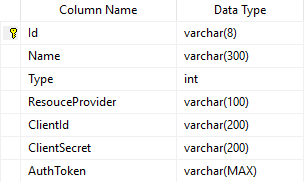
\includegraphics[width=0.7\linewidth]{images/schemaDB}
	\caption{Struttura tabella Organization del database}
	\label{fig:schemadb}
\end{figure}

\begin{itemize}
	\item \textbf{Id} : è un identificativo univoco alfanumerico, marcato come \textit{primary key} per poter distinguere i dati di  un'applicazione CRM di una specifica azienda;
	\item \textbf{Name} : è il nome del software CRM (eg. SalesForce o Dynamics);
	\item \textbf{Type} : è un campo intero per distinguere la tipologia di CRM (eg. SalesForce o Dynamics)  
	\item \textbf{ResoureProvider} :
	Ogni software CRM \textit{cloud-based} viene \glo{hostato} su un server, e per identificare a quale di questi ci si dovrà collegare bisogna anteporre a
	\item \textbf{ClientId} : è l’identificativo univoco (pubblico) del client ed è uno dei dati fondamentali che le applicazioni CRM devono fornire per permettere il collegamento di terze applicazioni-web tramite procedura OAuth;
	\item \textbf{ClietSecret} :  è l’identificativo segreto del client ed è il secondo dato fondamentale che le applicazioni CRM devono fornire per permettere il collegamento di terze applicazioni-web tramite procedura OAuth;
	\item \textbf{AuthToken} : è il campo contenente la risposta \glo{JSON} restituita da un CRM dopo la procedura di autenticazione OAuth; quindi non solo conterrà il \glo{token} da allegare per poter fare le richieste, ma anche il \glo{token} di refresh ed altri dati. Ne segue un esempio.
	
	
	\begin{lstlisting}[language=json,firstnumber=1]
	{
	"id":"https://login.salesforce.com/***",
	"issued_at":"1278448101416",
	"refresh_token":"***",
	"instance_url":"https://***.salesforce.com/",
	"signature":"***",
	"access_token":"***"
	}
	\end{lstlisting}
	
\end{itemize}


\subsection{Diagramma di sequenza}
	\begin{figure}[H]
	\centering
	\rotatebox{90}{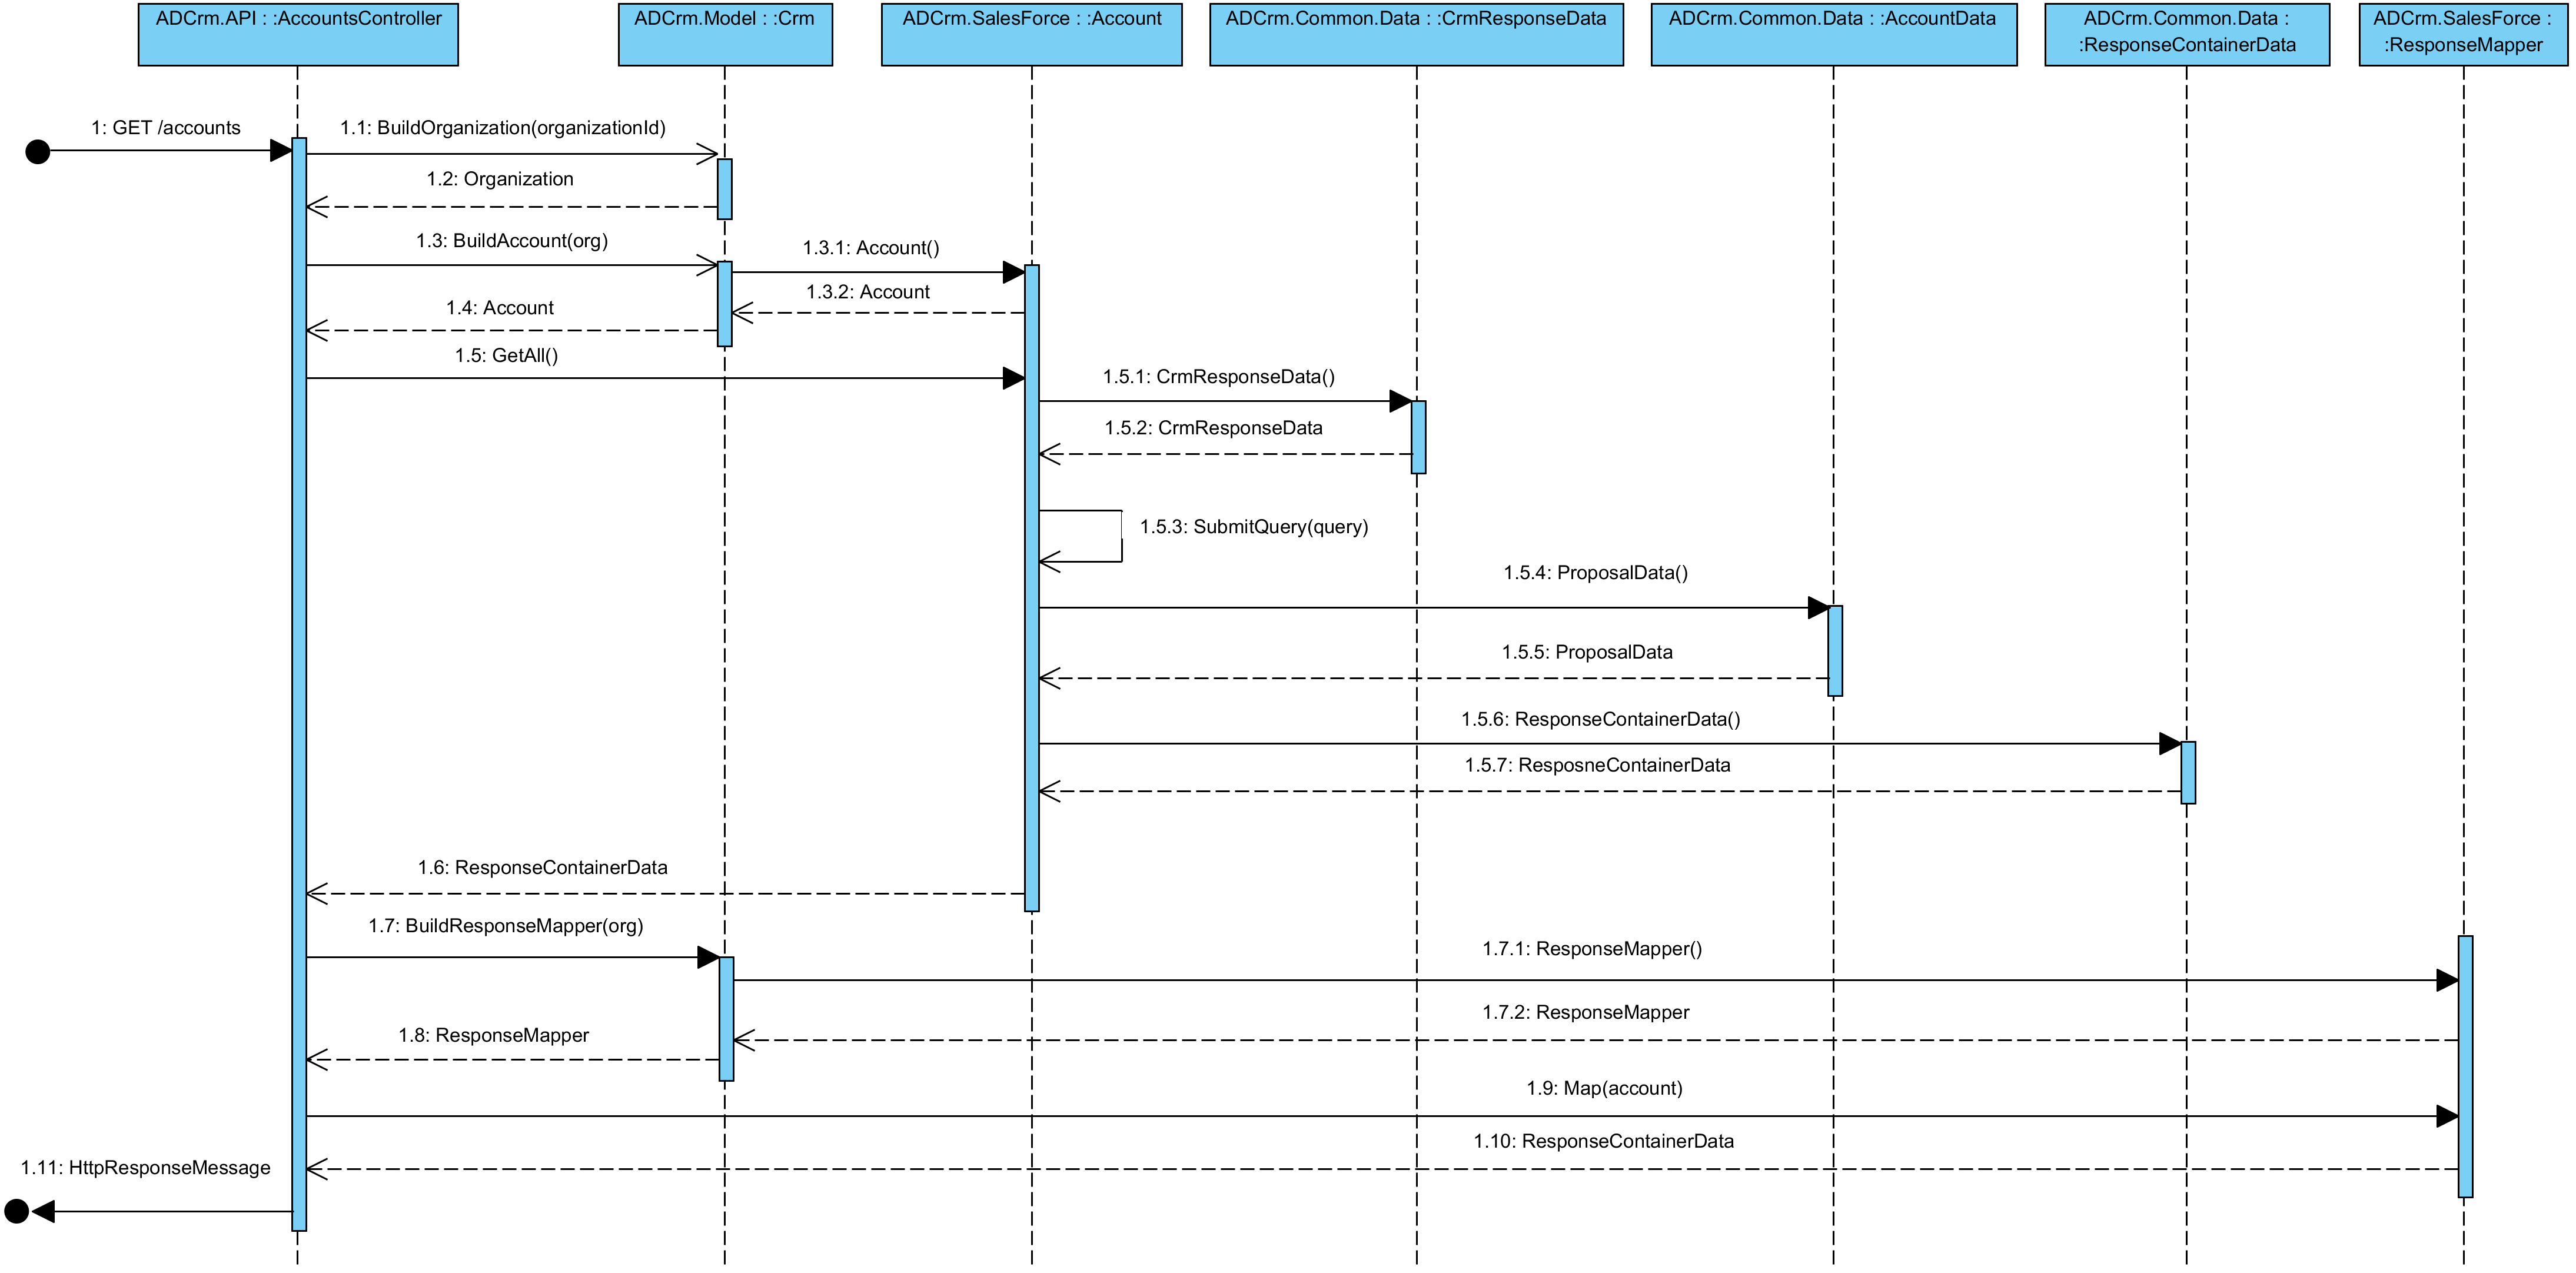
\includegraphics[width=\textheight,height=1.08\linewidth]{images/sdProposals}}
	
	\caption{Diagramma di sequenza per una chiamata per recuperare le proposte commerciali da un CRM }
	\label{fig:sdProposals}
\end{figure}


\chapter{Verifica e validazione}\label{verifica_validazione}

\chapter{Conclusioni}\label{conclusioni}

%**************************************************************
% Glossary and bibliography
%**************************************************************
\printglossaries
\bibliographystyle{unsrt}
%\bibliography{thesis}


%**************************************************************
% Ringraziamenti
%**************************************************************

%\chapter*{Thanksgivings}
%rr 

%\noindent\textit{\myLocation, \myTime}
%\hfill \myName
%\endgroup
\end{document}